\chapter{Chapter 4}

In this final chapter we will first introduce reaction-diffusion equations in continuous and discrete domains. We will then present a hierarchy of progressively more sophisticated architectures to emulate such systems. We will test these architectures on a simple one dimensional system and on the FH two-dimensional model on a BA network. Finally, we will introduce a method to extract the phase diagram of the reaction potentials of these equations purely from data.

\section{Problem definition}
\subsection{Reaction-diffusion dynamics on complex networks}

Reaction-Diffusion (RD) systems constitute a cornerstone of mathematical physics, 
providing a fundamental framework to describe processes where the distribution of substances changes due to two competing mechanisms: 
local chemical reactions and spatial diffusion. Classically defined on continuous Euclidean domains $\Omega \subset \mathbb{R}^d$, 
these systems are governed by parabolic partial differential equations of the form:
\begin{equation}
    \frac{\partial \mathbf{u}}{\partial t} = \nu \Delta \mathbf{u} + \mathbf{f}(\mathbf{u}),
\end{equation}
where $\mathbf{u}(\mathbf{x},t)$ represents the state vector (e.g., chemical concentrations), $\nu$ is the diffusion coefficient, $\Delta = \nabla^2$ is the
Laplacian operator representing spatial diffusion, and $\mathbf{f}(\mathbf{u})$ describes the non-linear reaction kinetics. 
These dynamics are renowned for generating complex spatio-temporal patterns, such as Turing patterns, traveling waves, and spirals \cite{turing1952chemical,nakao2010turing}

Recent advances in Operator Learning have focused on learning these dynamics efficiently in continuous domains. Notably, Wang and Hao \cite{wang2025laplacian} proposed 
a \textit{Laplacian Eigenfunction-Based Neural Operator} (LE-NO). Their approach exploits the spectral decomposition of the continuous 
Laplacian to efficiently approximate the non-linear reaction term, demonstrating that spectral information is critical for learning accurate operators in 
reaction-diffusion problems.

However, many real-world complex systems—such as social networks, connectomes, and power grids—are 
intrinsically discrete and topologically irregular. On these \textit{Complex Networks}, 
the notion of continuous space is replaced by a graph topology $\mathcal{G} = (\mathcal{V}, \mathcal{E})$, consisting of $N$ nodes. Consequently, 
the continuous Laplacian operator is replaced by the \textbf{Graph Laplacian matrix} $\mathbf{L} \in \mathbb{R}^{N \times N}$, defined as:
\begin{equation}
    \mathbf{L} = \mathbf{D} - \mathbf{A},
\end{equation}
where $\mathbf{A}$ is the adjacency matrix and $\mathbf{D}$ is the diagonal degree matrix. The reaction-diffusion dynamics on the network are then governed by a system of coupled Ordinary Differential Equations (ODEs):
\begin{equation}
    \frac{d \mathbf{U}}{dt} = - \nu \mathbf{L} \mathbf{U} + \mathbf{F}(\mathbf{U}),
    \label{eq:react_diff_on_net}
\end{equation}
where $\mathbf{U}(t) \in \mathbb{R}^{N \times d_u}$ is the state of all nodes at time $t$. The term $- \mathbf{L} \mathbf{U}$ captures the diffusion process across the edges of the graph, driving the system towards consensus, while $\mathbf{F}(\mathbf{U})$ applies the non-linear reaction independently at each node.

While the spectral properties of $\mathbf{L}$ are well-studied in network science, the application of Operator Learning to predict these dynamics on complex graphs 
remains underexplored. 
The shift from the continuous paradigm to the discrete domain has diverse implications. For instance the advantage of Operator architectures becomes less clear, since we don't have anymore a continuous domain on which we can exploit the discretization-invariance property. However, we believe that this feature could be still useful when analyzing networks of varying sizes.
Specifically, the challenge lies in whether Neural Operators can effectively learn these dynamics "blindly" from nodal time-series, 
or if explicitly informing the network with the spectral geometry of $\mathbf{L}$ (via its eigendecomposition) provides a necessary inductive bias for generalization.

% Questo lo lascio alla fine come spunto futuro ?
Another interesting aspect, that is an original contibution of this thesis, is the possibility to derive a phase portrait from the distribution of $\mathbf{F}(\mathbf{U})$ learned by the neural network.

\section{Methodology}

\subsection{Problem formulation}
We consider a dynamical system defined on a graph $\mathcal{G} = (\mathcal{V}, \mathcal{E})$, whose state $\mathbf{u}(t) \in \mathbb{R}^N$ evolves
according to Eq. \eqref{eq:react_diff_on_net}. 
Our aim was to predict an approximation of the \textbf{time-stepper operator} $\Psi_{\Delta t}$, which maps the system state from time $t$ to time $t + \Delta t$.
%on an undirected, connected graph $\mathcal{G} = (\mathcal{V}, \mathcal{E})$ with $N = |\mathcal{V}|$ nodes. 
%The state $\mathbf{u}(t) \in \mathbb{R}^N$ evolves according to a semi-linear PDE discretized on the graph:


\subsubsection{Experimental design: hierarchy of inductive bias}
\label{sec:exp_design}
To systematically evaluate the impact of physical and topological information on learning performance, we compared three architectures with increasing levels of "inductive bias".

\subsubsection{Level 1: totally blind (black-box)}
This baseline represents the purely data-driven approach. The model ignores both the diffusion physics and the graph topology. It attempts to learn the discrete time-stepper operator $\Psi_{\Delta t}$ end-to-end:
\begin{equation}
    \mathbf{u}^{n+1} \approx \text{Net}_{\theta}(\mathbf{u}^n)
\end{equation}
Here, the network must implicitly learn both the diffusion operator $-\nu \mathbf{L}$ and the reaction operator $\mathbf{F}$ simultaneously from data. This implies that the network must statistically reconstruct the graph structure solely from the propagation of signals, a task that typically requires massive amounts of training data. Moreover, we decided, to compare the same families of architectures and further analyze the importance of using topological information for the prediction, to use continuous operator network, which required us to embed the graphs in a continuous spatial domains. This first level is the only approach which does not require topological information.

\subsubsection[Level 2: physics-informed (hybrid nodal)]{Level 2: Physics-Informed\footnote{We chose this name given the strong connection with the Physics Informed Neural Networks (PINNs) family.} (Hybrid Nodal)}
In this approach, we injected physical knowledge by using an \textbf{Implicit-Explicit (IMEX)} solver \footnote{see Appendix \ref{app:C}.}. We assume the linear diffusion term $-\nu \mathbf{L}$ is known, and the network is tasked \textit{only} with approximating the reaction term $\mathbf{F}(\mathbf{u})$.

The update rule enforces the diffusion physics exactly:
\begin{equation}
    (\mathbf{I} + \Delta t \nu \mathbf{L}) \mathbf{u}^{n+1} = \mathbf{u}^n + \Delta t \cdot \text{Net}_{\theta}(\mathbf{u}^n)
    \label{eq:imex_update}
\end{equation}
%While "Physics-Informed", this model remains \textbf{"Topologically Blind"} regarding the reaction learning: the network approximates $\mathbf{F}(\mathbf{u})$ node-wise using a normalized coordinate system, ignoring the graph's symmetries and spectral clusters.


%

%\newline 
While the diffusion coefficient $\nu$ can be treated as a known physical prior, it can also be discovered directly from observational data. In our experiments, we cast this as a joint system identification problem: $\nu$ is initialized as a differentiable scalar variable and optimized end-to-end alongside the neural network weights $\theta$ via gradient descent.
It is worth noting that the neural network $\text{Net}_{\theta}(\mathbf{u})$ remains \textbf{"topologically blind"}. As in Level 1, it relies on embedding the discrete graph into an artificial continuous domain. However, this limitation is less detrimental in this hybrid formulation: since the target reaction term is strictly local (acting node-wise), explicitly capturing the spatial relations between nodes becomes less critical for the network. Nevertheless, this architectural flaw will be fully addressed in Level 3.

\subsubsection{Level 3: topology-informed (hybrid spectral)}
Here the model leveraged both physical and topological priors.
The diffusion operator was enforced exactly via the IMEX scheme as in Level 2.

Although the "Physics-Informed" approach ensures that the linear diffusion process is efficiently resolved by the numerical solver, the neural network $\text{Net}_{\theta}$ responsible for learning the non-linear reaction remains fundamentally \textbf{"topologically blind"}. While the exact mathematical formulation of the reaction term $\mathbf{F}(\mathbf{U})$ is intrinsically local (acting node-wise), learning this operator from observational data poses a severely ill-posed inverse problem. The temporal snapshots $\mathbf{u}^n$ embed global spatial correlations generated by the continuous diffusion process, and numerical approximations of time-derivatives inevitably amplify high-frequency noise. If $\text{Net}_{\theta}$ relies on a standard node-wise Multilayer Perceptron (MLP) or conventional operator architectures (such as standard FFT-based Fourier Neural Operators or Euclidean DeepONets), it processes the state variables using arbitrary or grid-based coordinates. Consequently, it completely ignores the true connectivity, symmetries, and spectral clusters of the complex network, making the learning process susceptible to local noise and spatial overfitting. To robustly decouple the local reaction kinetics from the inherent noise, it is necessary to explicitly embed the topological information of the Graph Laplacian $\mathbf{L}$ directly into the neural architecture. By doing so, for instance by using Laplacian eigenvectors to define the spectral layer in a LFNO, or substituting the trunk network of a DeepONet with Laplacian eigenfunctions as proposed in continuous domains by Wang and Hao \cite{wang2025laplacian}, the learning process is projected onto the graph's intrinsic, low-dimensional spectral manifold. This topological injection acts as a powerful structural prior: it regularizes the optimization landscape, naturally filters out non-physical, topology-violating noise, and enables the model to accurately recover the underlying local kinetics from globally coupled observations.
%However, the neural network approximated the reaction term in the \textit{graph spectral domain}, utilizing the eigenbasis $\mathbf{\Phi}$ of the Graph Laplacian $\mathbf{L}$.

\begin{comment}
One of our proposed methods, the \textbf{Laplacian Eigenfunction Neural Operator (LENO) on Network}, incorporates both physical and topological priors.
It operates in a \textit{truncated} spectral domain defined by the eigenvectors of the Laplacian.
Specifically, we select the matrix $\mathbf{\Phi}_p \in \mathbb{R}^{N \times p}$ containing only the eigenvectors corresponding to the $p$ smallest eigenvalues $0 \le \lambda_1 \le \dots \le \lambda_p$ (low-frequency modes), where $p < N$ is a hyperparameter chosen during training.

\begin{enumerate}
    \item \textbf{Projection:} Inputs are projected to low-dimensional spectral coefficients $\boldsymbol{\beta}^n = \mathbf{\Phi}_p^T \mathbf{u}^n \in \mathbb{R}^p$.
    \item \textbf{Learning:} A Network predicts the spectral residual of the reaction term: $\hat{\mathbf{R}} = \text{Net}_{\theta}(\boldsymbol{\beta}^n)$.
    \item \textbf{Update:} The next state is computed via the exact spectral IMEX scheme for the first $p$ modes:
    \begin{equation}
        \beta_k^{n+1} = \frac{\beta_k^n + \Delta t \hat{R}_k}{1 + \Delta t \nu \lambda_k}, \quad k=1,\dots,p
    \end{equation}
    The physical state is finally reconstructed as $\mathbf{u}^{n+1} \approx \mathbf{\Phi}_p \boldsymbol{\beta}^{n+1}$.
\end{enumerate}
%This model is \textbf{"Fully Informed"}: it leverages the exact solver for diffusion and the truncated native eigenbasis of the graph for efficient representation.
It is important to note that, since we posed the problem in the right coordinates, usually a simple MLP suffices to learn the coupling between modes, 
without the need for complex architectures (as we will see in the next section).
\end{comment}


\subsection{Training objective: composite loss strategy}
For the informed architectures (Levels 2 and 3), the learning task has been reframed: instead of predicting the state evolution directly, the networks approximated the non-linear reaction term $\mathbf{F}(\mathbf{u})$. To ensure both temporal stability and physical consistency, we employed a composite loss function consisting of two terms:
 a \textbf{Trajectory Loss} and a \textbf{Physics (Residual) Loss}.


\subsection{Ground truth reaction extraction}
Since the dataset contains state snapshots $\mathbf{u}$ but not explicit values for the reaction $\mathbf{F}(\mathbf{u})$, we first extracted the "ground truth" reaction target, denoted as $\mathbf{R}_{GT}$, by inverting the numerical scheme used for data generation.
Given the IMEX structure, the effective reaction responsible for the transition $\mathbf{u}^n \to \mathbf{u}^{n+1}$ is:
\begin{equation}
    \mathbf{R(u)}_{GT}^n = \underbrace{\frac{\mathbf{u}^{n+1} - \mathbf{u}^n}{\Delta t}}_{\text{Finite Difference}} + \underbrace{\nu \mathbf{L} \mathbf{u}^{n+1}}_{\text{Implicit Diffusion}}
\end{equation}
For Level 3, the target was the approximation $\mathbf{{R}_{GT}}^{n}_{p} = \mathbf{\Phi}_p^T \mathbf{R}_{GT}^n \mathbf{\Phi}_p$, or the projection onto the spectral domain: ${\hat{\mathbf{R}}_{GT}}^{n}_{p} = \mathbf{\Phi}_p^T \mathbf{R}_{GT}^n$, where the matrix $\mathbf{\Phi}_p \in \mathbb{R}^{N \times p}$ contains only the eigenvectors corresponding to the $p$ smallest eigenvalues $0 \le \lambda_1 \le \dots \le \lambda_p$ (low-frequency modes).

\subsubsection{Loss components}
The total loss $\mathcal{L}$ was defined as a weighted sum:
\begin{equation}
    \mathcal{L} = \mathcal{L}_{traj} + \lambda_{phys} \mathcal{L}_{phys}
\end{equation}
where $\lambda_{phys}$ is a balancing hyperparameter \footnote{in our experiments, we tuned $\lambda_{phys}$ as an hyperparameter of the model, before training.}
\footnote{For the blind architectures we used only the trajectory loss.}.

\begin{enumerate}
    \item \textbf{Physics (residual) loss ($\mathcal{L}_{phys}$):} 
    This term provided instantaneous supervision, forcing the neural network $\text{Net}_\theta$ to learn the local physical law governing the reaction.
\begin{equation}
    \mathcal{L}_{phys} = \frac{1}{N_{res}} \sum_{j=1}^{N_{res}} \| \text{Net}_\theta(\mathbf{x}_j) - \mathbf{R}_{GT}(\mathbf{x}_j) \|_2
\end{equation}
where $\mathbf{x}_j = \mathbf{u}_j^{m\left( j \right)}$ represents a single state snapshot for the $j$-th sample at a randomly sampled time step $m$ (different for each $j$) and $N_{res}$ is the batch size for the physical loss. Inputs $\mathbf{x}$ and targets $\mathbf{R}$ can be in nodal space or in spectral space (only for LENO).
\newline
    It is worth noting that this term acted analogously to the PDE residual loss ($\mathcal{L}_{PDE}$) found in classical Physics-Informed Neural Networks (PINNs), as it penalizes deviations from the governing equation.
    \footnote{However, unlike standard PINNs where the entire PDE is enforced via optimization (soft constraint), our hybrid framework enforced the diffusion
     operator exactly via the numerical architecture (hard constraint), leaving the loss function responsible solely for the reaction dynamics.}

\item \textbf{Relative trajectory loss ($\mathcal{L}_{traj}$):}
This term measured the relative error of the integrated next-step state. Normalizing by the ground truth magnitude ensured the loss is scale-invariant and prevented the model from biasing towards high-amplitude regions.
\begin{equation}
    \mathcal{L}_{traj} = \frac{1}{N_{traj} N_T} \sum_{i=1}^{N_{traj}} \sum_{n=0}^{N_T-1} \frac{\| \Psi_{\Delta t}(\hat{\mathbf{u}}^n_i, \theta) - \mathbf{u}^{n+1}_{true, i} \|_2}{\| \mathbf{u}^{n+1}_{true, i} \|_2 + \epsilon}
\end{equation}
where $\Psi_{\Delta t}$ represents the differentiable IMEX solver layer, $\hat{\mathbf{u}}^n_i$ is the predicted state at step $n$ (with $\hat{\mathbf{u}}^0_i = \mathbf{u}^0_{true, i}$), $\epsilon=10^{-6}$ is a small constant for numerical stability, $N_{traj}$ is the batch size for the trajectory, and $N_T$ is the total number of time steps.

    For the trajectory term we considered the relative L2 term for scale-invariance and better interpretability. However, during training, 
    we found that using the absolute L2 norm for the physics term provided better convergence properties \footnote{This particular choice depends on the specific problem. In section \ref{sec:Example 2} we used the relative loss also for the physics term.}.
\end{enumerate}



\subsection{Neural architectures implementation}

We instantiated the hierarchy of inductive biases defined in Sec. \ref{sec:exp_design} using the following specific architectures. All models were implemented in PyTorch.

\begin{itemize}
    \item \textbf{Level 1: black-box baselines.} (see Chapter \ref{Chp:2}) %Devo ancora creare la sezione di introduzione su ML e Neural Operators
    \begin{itemize}
        \item \textbf{Blind DeepONet:} In this baseline implementation, a \textit{Branch Net} (MLP) encoded the full global state vector, while a \textit{Trunk Net} (MLP) evaluated spatial basis functions at normalized coordinates $y \in [0,1]$. Crucially, these coordinates were assigned based solely on the node's arbitrary position within the 1D input data array (effectively mapping the $i$-th node in the dataset to the spatial coordinate $i/N$). By computing the final prediction through the dot product of these latent features, the architecture forced the discrete complex network onto a continuous 1D Euclidean domain. Consequently, it treated the graph nodes as uniformly spaced points on a line, restricting their spatial proximity to their arbitrary data storage order rather than their true topological connectivity.
        \item \textbf{Blind FNO:} A standard Fourier Neural Operator relying on the Fast Fourier Transform (FFT).
        Since the standard FFT cannot operate directly on non-Euclidean graph domains, the baseline FNO treated the node features as a flattened 1D sequence. This implicitly forced the network onto a uniformly spaced closed loop, where nodes are artificially connected based solely on their arbitrary array indices, completely ignoring the true graph topology.
         We truncated the frequency modes passed.
    \end{itemize}


\item \textbf{Level 2: physics-informed (hybrid)}\\
This tier decoupled physical laws from topological structure. Both architectures leveraged the \textbf{exact Graph-Spectral IMEX solver} for time-stepping, ensuring perfect diffusion dynamics via the true Graph Laplacian eigenvalues. However, the neural networks approximating the reaction term $\mathcal{N}(u)$ remained \textbf{topologically blind}, treating the graph signal as an Euclidean sequence.
\begin{itemize}
    \item \textbf{PI-DeepONet:} Utilized the standard Branch/Trunk architecture (same architecture as in level 1) to map the full state vector to the reaction residual.
    % It acted node-wise without explicit neighborhood information.
    \item \textbf{PI-FNO:} Used the FNO backbone (same architecture as in level 1) to predict the reaction vector. 
\end{itemize}

    \item \textbf{Level 3: topology-informed (spectral).}
    \begin{itemize}
        \item \textbf{Laplacian Eigenfunction Neural Operator (LENO) on network:} 
        This method operated in a \textit{truncated} spectral domain defined by the eigenvectors of the Laplacian.
Specifically, we selected the matrix $\mathbf{\Phi}_p \in \mathbb{R}^{N \times p}$ containing only the eigenvectors corresponding to the $p$ smallest eigenvalues $0 \le \lambda_1 \le \dots \le \lambda_p$ (low-frequency modes), where $p < N$ is a hyperparameter chosen during training.

\begin{enumerate}
    \item \textbf{Projection:} Inputs were projected to low-dimensional spectral coefficients $\boldsymbol{\beta}^n = \mathbf{\Phi}_p^T \mathbf{u}^n \in \mathbb{R}^p$.
    \item \textbf{Learning:} A Network predicted the spectral residual of the reaction term: $\hat{\mathbf{R}} = \text{Net}_{\theta}(\boldsymbol{\beta}^n)$.
    \item \textbf{Update:} The next state was computed via the exact spectral IMEX scheme for the first $p$ modes:
    \begin{equation}
        \beta_k^{n+1} = \frac{\beta_k^n + \Delta t \hat{R}_k}{1 + \Delta t \nu \lambda_k}, \quad k=1,\dots,p
    \end{equation}
    The physical state was finally reconstructed as $\mathbf{u}^{n+1} \approx \mathbf{\Phi}_p \boldsymbol{\beta}^{n+1}$.
\end{enumerate}
%This model is \textbf{"Fully Informed"}: it leverages the exact solver for diffusion and the truncated native eigenbasis of the graph for efficient representation.
It is important to note that, since we posed the problem in the right coordinates, usually a simple MLP suffices to learn the coupling between modes, 
without the need for complex architectures.

    \item \textbf{Graph (Laplacian)-FNO (ours):} It operated in a similar way to LENO.
    However it built on the standard FNO, so it replaced FFT/IFFT operations with the Graph Fourier Transform (GFT, where the input is projected onto the first $p$ eigenvectors of the Graph Laplacian ($\mathbf{\Phi}_p$)).
    
   The primary distinction between LFNO and LENO lies in the domain where the objective function is evaluated. While LENO minimizes the error directly on the transformed spectral coefficients, LFNO projects the latent representation back into the physical space via the inverse GFT, penalizing the reaction term directly at the nodal level.
    
        
        
%The proposed spectral residual learner. 
%Unlike deep FNOs, the core reaction approximation is handled by a concise MLP operating directly on the spectral coefficients $\boldsymbol{\beta}$, 
%leveraging the exact IMEX solver for the diffusion update.
    \end{itemize}
\end{itemize}

%\paragraph{Implementation Note.} 
%A key distinction from classical PINNs lies in constraint enforcement. While PINNs minimize the PDE residual as a soft loss term ($\mathcal{L}_{PDE}$), our Level 3 framework enforces the diffusion operator exactly via the numerical architecture (hard constraint) as shown in Eq. (\ref{eq:imex_update}). This strictly reduces the hypothesis space to physically valid diffusion processes on the graph.

%%%%%%%%%%%
\subsection{Training details}
All models were implemented in PyTorch and trained on an NVIDIA Quadro RTX 5000 GPU. To ensure reproducibility, fixed random seeds ($42$) were used for all experiments.

The network parameters were optimized using the Adam algorithm with a weight decay of $10^{-4}$ and a gradient clipping threshold of $1.0$ to ensure numerical stability
\footnote{Only for levels $2\&3$, since the loss can be more prone to stiffness and exploding gradients due to the inclusion of physical constraints and solver dynamics.}.
% We employed a mini-batch strategy with a batch size of $128$ for the trajectory data.

To select the optimal configuration, we performed an automated hyperparameter search using the \textit{Optuna} framework. To efficiently explore the search space, we utilized a \textit{Median Pruner} to early-stop unpromising trials. The search space included common parameters across all models and architecture-specific ones:
\begin{itemize}
    \item Learning rate: $\eta \in [10^{-5}, 5\cdot 10^{-3}]$ (log-uniform sampling);
    \item Physics penalty weight \footnote{Only for levels $2\&3$\label{fn:levels}}: $\lambda_{\text{phys}} \in [10^{-5}, 10.0]$ (log-uniform sampling);
    \item Initial guess for square root of the diffusion coefficient ($\nu= \varepsilon^2$)\textsuperscript{\ref{fn:levels}}: $\varepsilon_{\text{init}} \in [0.5, 2.0]$;
    \item Architecture-specific hyperparameters (e.g., hidden layer width, number of modes) were optimized within ranges appropriate for each specific model.
\end{itemize}

Once the best hyperparameters were identified, the final models were trained for $500$ epochs. The learning rate was scheduled to decrease by a factor of $\gamma = 0.5$ every $300$ epochs. 
To prevent overfitting, we monitored the error on a validation set and saved the model weights and fitted $\epsilon$, corresponding to the epoch with the lowest validation loss.

\section{Example 1: Allen-Cahn on graph (hierarchy of inductive bias)}

\subsection{Data generation}
To evaluate the proposed methods, we simulated the \textbf{Allen-Cahn equation} on a complex network. 
%The Allen-Cahn equation is a well-known reaction-diffusion model used in phase-transition problems.

%%%%%%%%%%%%%%%%%%%%%%%%%%%
The Allen-Cahn equation describes a reaction-diffusion process governed by the gradient flow of a Ginzburg-Landau free energy functional~\cite{allen1979microscopic}.
 While its primary application lies in predicting microstructural evolution during phase transitions in materials~\cite{chen2002phase},
  its ability to drive systems toward stable stationary states makes it a versatile tool. 
  Applications range from geometrical image segmentation~\cite{benes2004geometrical} to finding minimal cuts in graph theory and analyzing community structures
   in complex networks~\cite{bertozzi2012diffuse}.
%%%%%%%%%%%%%%%%%%%%%%%%%%%%
\subsection{Graph topology}
We generated a scale-free network using the \textbf{Barabási-Albert (BA)} model to mimic realistic topological features such as hubs and clusters.
\begin{itemize}
    \item \textbf{Nodes:} $N = 1000$.
    \item \textbf{Attachment:} $m = 2$ (each new node attaches to 2 existing nodes).
\end{itemize}

\subsection{Dynamics: Allen-Cahn on graphs}
The specific form of the reaction term for the Allen-Cahn equation is cubic:
\begin{equation}
    \mathbf{F}(\mathbf{u}) = \mathbf{u} - \mathbf{u}^3
\end{equation}
The system evolved from an initial condition of $50$, randomly selected, active nodes.
We generated a training dataset of $15000$ trajectories ($10000$ for training, $3000$ for validation and $2000$ for testing) by numerically integrating the system using 
a spectral IMEX solver \footnote{details in Appendix \ref{app:C}.},
 subsampling the snapshots at time intervals $\Delta=0.05 t$ for 21 time steps to create the input-target pairs. In Figure \ref{fig:experimental_design} we can observe the evolution of the node dynamics.

\begin{figure}
    \centering
    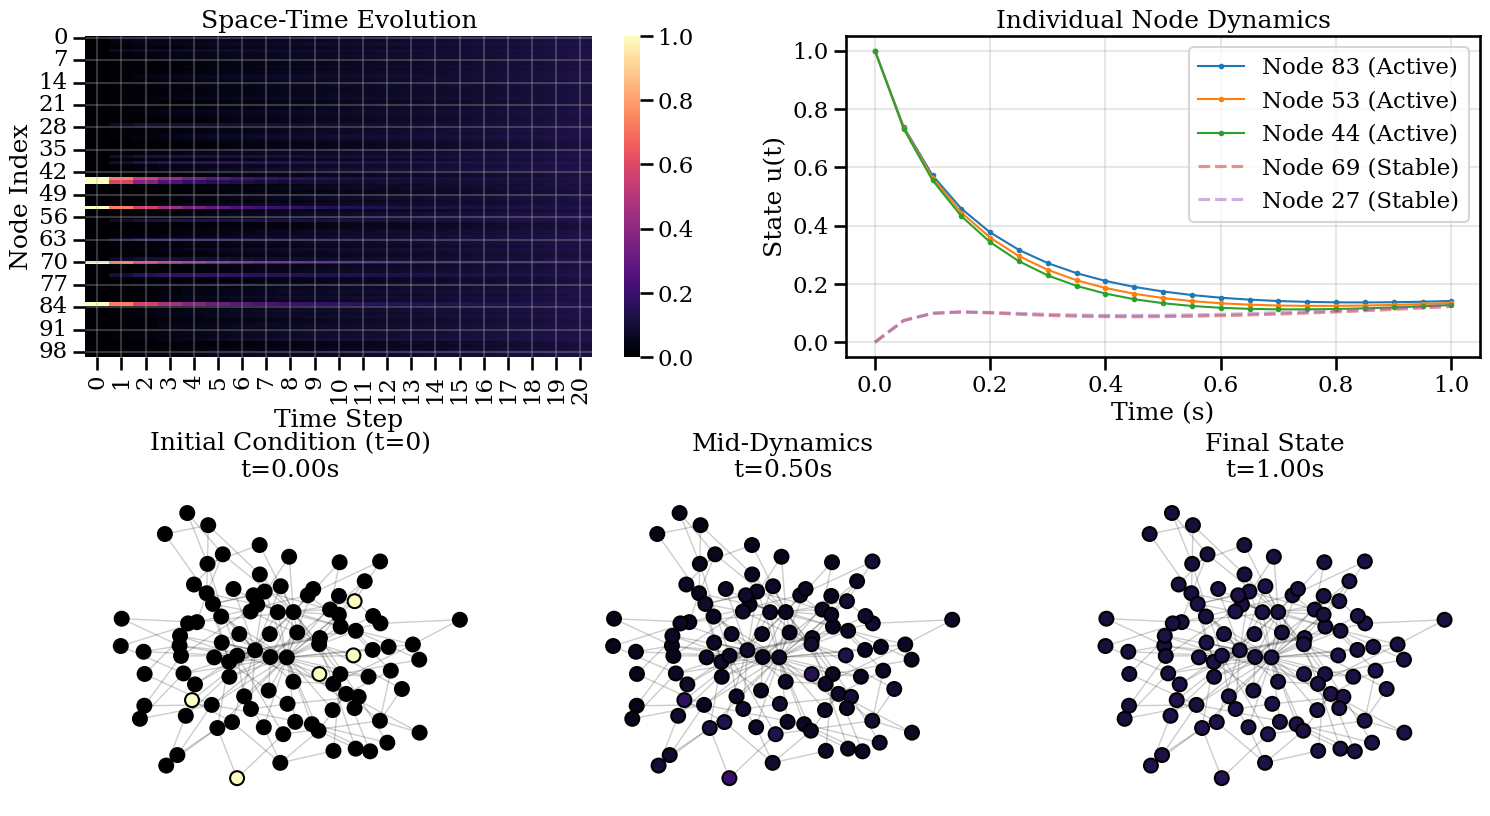
\includegraphics[width=1.0\textwidth]{img/Allen-Cahn/dynamics_Allen_Cahn_v2.png}
    \caption{Simulation of Allen-Cahn dynamics on a Barabási-Albert graph with $N=100$ nodes and $m=2$. The figure illustrates the evolution of all node states (top left, bottom) over time, and a focus on some representative nodes (top right), showcasing both the reaction and diffusive processes.}
    \label{fig:experimental_design}
\end{figure}

%%%%%%%%%

\subsection{Results and discussion}

\subsubsection{Quantitative analysis: error distribution}
We begin our analysis by examining the distribution of the relative $L_2$ errors on the test set (2000 trajectories). 
Figure \ref{fig:error_matrix} presents a systematic comparison of the test errors arranged by model family (columns) and inductive bias level (rows).
On the other hand Figure \ref{fig:heatmap_vertical_stack} shows an absolute error comparison between the same models, however it rearranges the two columns representing the families of architectures on the same page.

This visualization highlights the progressive improvement in generalization performance as we move from "Blind" models to "Topology-Informed" architectures.

%%%%%%%%%%%%%%%%%%%%%%%%%%%%%%
\begin{figure}[htbp]
    % Usiamo makebox per centrare la figura sforando i margini della pagina
    \makebox[\textwidth][c]{%
        % Aumenta o diminuisci 1.15 per gestire la grandezza totale (1.15 = 115% della larghezza del testo)
        \begin{minipage}{1.4\textwidth} 
            
            % --- HEADERS ---
            \begin{minipage}{0.05\textwidth} 
                \hfill 
            \end{minipage}
            \hfill 
            \begin{minipage}{0.46\textwidth} 
                \centering \textbf{DeepONet Family}
            \end{minipage}
            \hfill 
            \begin{minipage}{0.46\textwidth} 
                \centering \textbf{FNO Family}
            \end{minipage}
            \par\medskip

            % --- ROW 1: LEVEL 1 (BLIND) ---
            \begin{minipage}[c]{0.05\textwidth}
                \centering 
                \rotatebox{90}{\parbox{2.5cm}{\centering \textbf{Level 1} \\ (Blind)}}
            \end{minipage}
            \hfill
            \begin{minipage}[c]{0.46\textwidth}
                \centering
                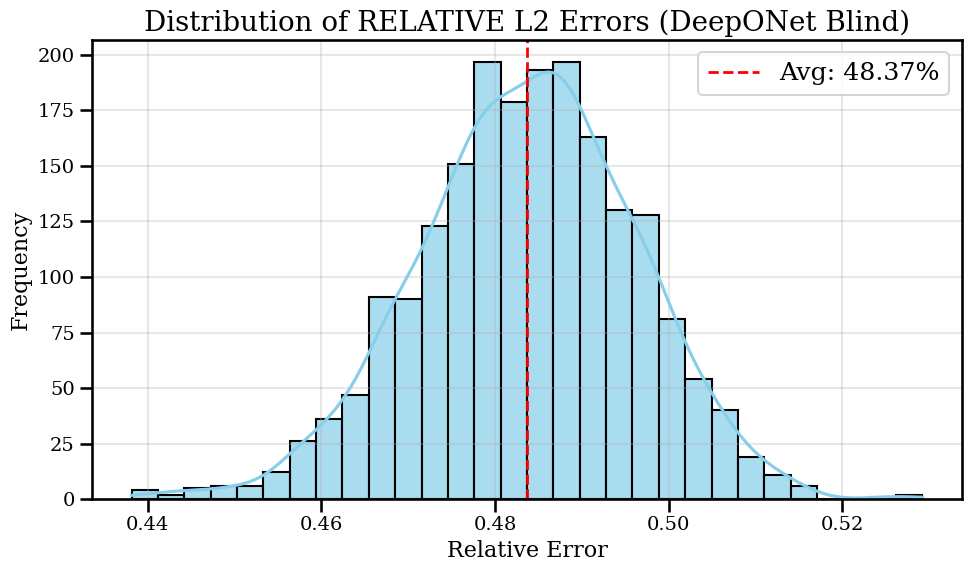
\includegraphics[width=\linewidth]{img/Allen-Cahn/Histograms/hist_test_set_deeponet_blind_v2.png}
            \end{minipage}
            \hfill
            \begin{minipage}[c]{0.46\textwidth}
                \centering
                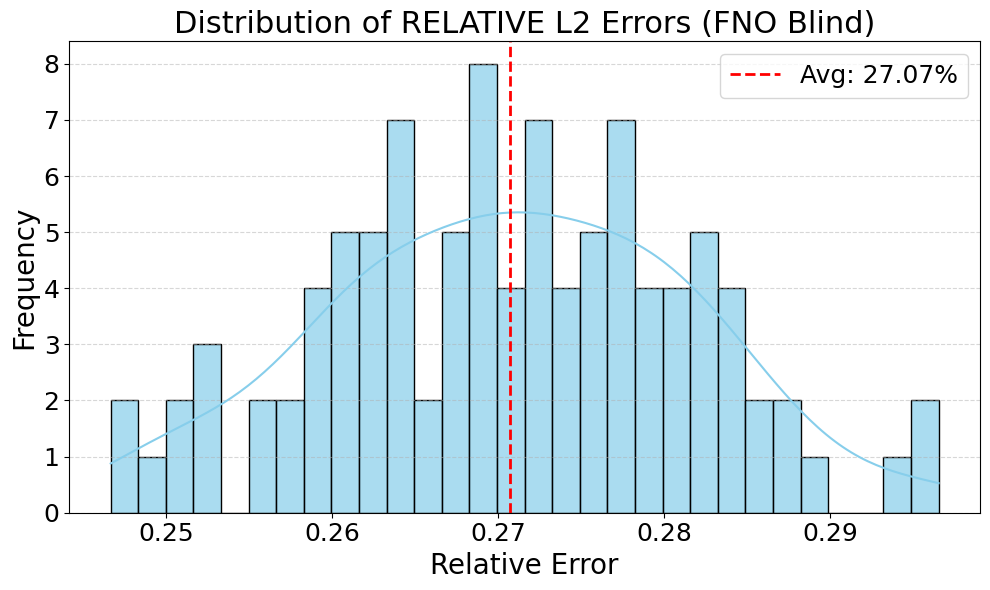
\includegraphics[width=\linewidth]{img/Allen-Cahn/Histograms/hist_test_set_FNO_blind_v2.png}
            \end{minipage}
            \par\bigskip 

            % --- ROW 2: LEVEL 2 (PHYSICS-INFORMED) ---
            \begin{minipage}[c]{0.05\textwidth}
                \centering 
                \rotatebox{90}{\parbox{2.5cm}{\centering \textbf{Level 2} \\ (Physics)}}
            \end{minipage}
            \hfill
            \begin{minipage}[c]{0.46\textwidth}
                \centering
                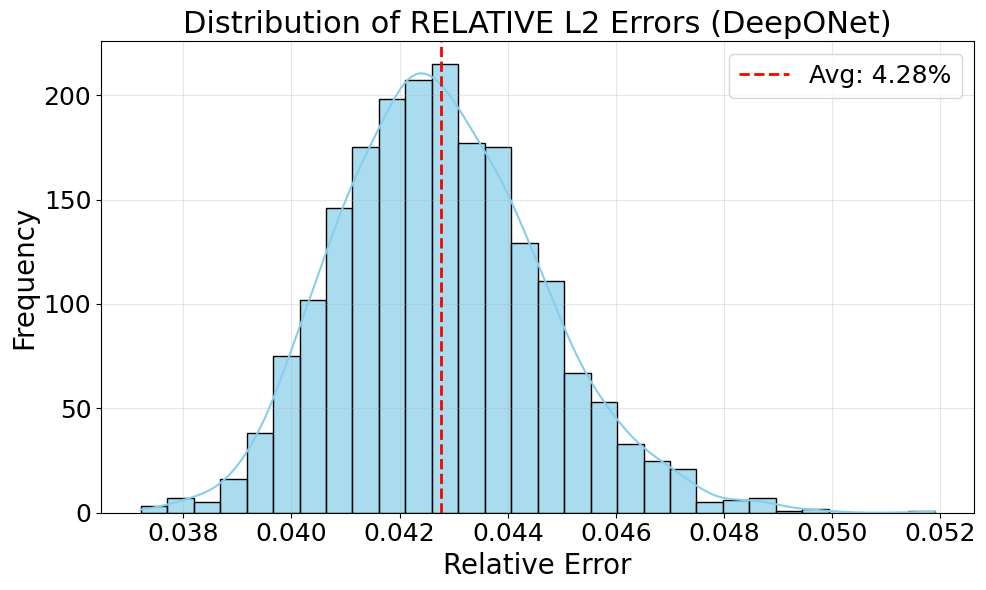
\includegraphics[width=\linewidth]{img/Allen-Cahn/Histograms/hist_test_set_deeponet_v2.png}
            \end{minipage}
            \hfill
            \begin{minipage}[c]{0.46\textwidth}
                \centering
                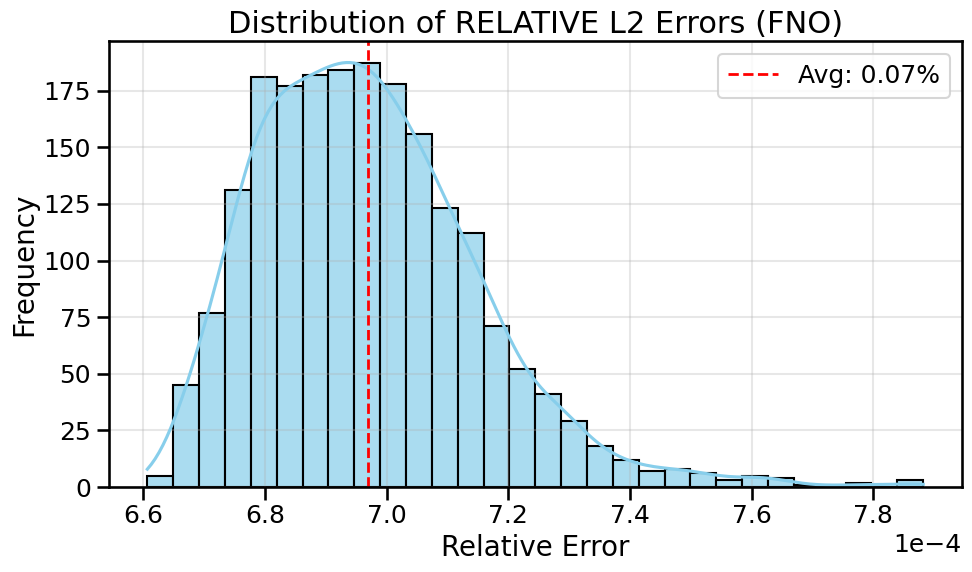
\includegraphics[width=\linewidth]{img/Allen-Cahn/Histograms/hist_test_set_FNO_v2.png}
            \end{minipage}
            \par\bigskip

            % --- ROW 3: LEVEL 3 (TOPOLOGY-INFORMED) ---
            \begin{minipage}[c]{0.05\textwidth}
                \centering 
                \rotatebox{90}{\parbox{2.5cm}{\centering \textbf{Level 3} \\ (Topology)}}
            \end{minipage}
            \hfill
            \begin{minipage}[c]{0.46\textwidth}
                \centering
                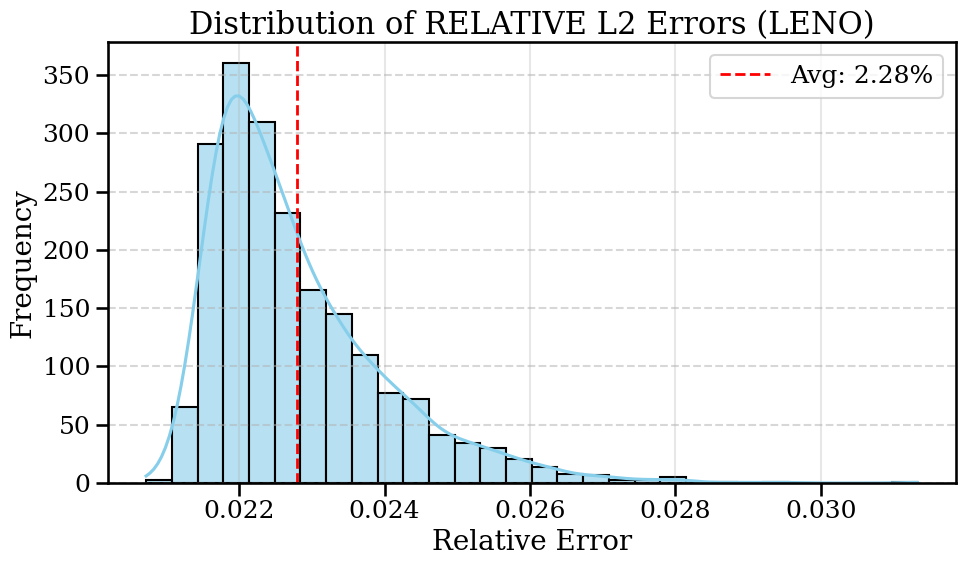
\includegraphics[width=\linewidth]{img/Allen-Cahn/Histograms/hist_test_set_leno_v2.png}
                \subcaption*{LENO}
            \end{minipage}
            \hfill
            \begin{minipage}[c]{0.46\textwidth}
                \centering
                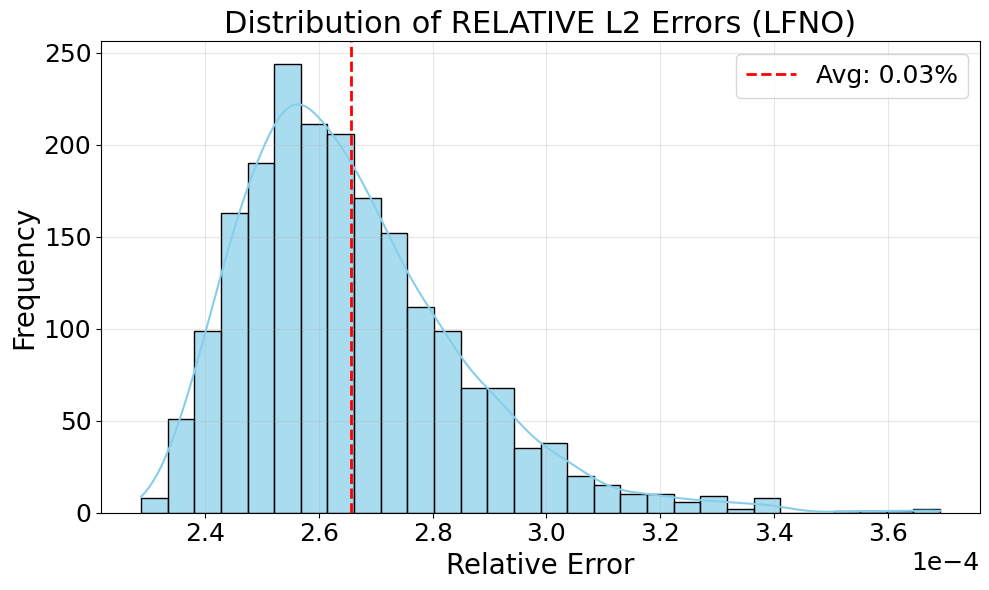
\includegraphics[width=\linewidth]{img/Allen-Cahn/Histograms/hist_test_set_LFNO_v2.png}
                \subcaption*{LFNO}
            \end{minipage}
            
        \end{minipage}
    } % Fine makebox
    
\caption{Matrix of Relative $L_2$ Error distributions on the test set.
    \textbf{Columns} distinguish between Nodal architectures (DeepONet family)%\protect\footnotemark 
     and Spectral architectures (FNO family). 
    \textbf{Rows} represent the hierarchy of inductive bias: Level 1 (Totally Blind), Level 2 (Physics-Informed), and Level 3 (Topology-Informed). 
    The red dashed line indicates the mean error. Note how the LFNO model (bottom right) achieves the lowest error variance and mean.}
    \label{fig:error_matrix}
\end{figure}



\begin{comment}
\begin{figure}[htbp]
    \centering
    
    % --- HEADERS (Struttura identica alle righe sotto) ---
    % 1. Spacer per l'etichetta verticale (0.05)
    \begin{minipage}{0.05\textwidth} 
        \hfill 
    \end{minipage}
    \hfill % <--- QUESTO MANCAVA! Allinea con lo spazio delle righe sotto
    % 2. DeepONet Title (0.46)
    \begin{minipage}{0.46\textwidth} 
        \centering \textbf{DeepONet Family}
    \end{minipage}
    \hfill % Spazio tra le due colonne principali
    % 3. FNO Title (0.46)
    \begin{minipage}{0.46\textwidth} 
        \centering \textbf{FNO Family}
    \end{minipage}
    \par\medskip

    % --- ROW 1: LEVEL 1 (BLIND) ---
    \begin{minipage}[c]{0.05\textwidth}
        \centering 
        \rotatebox{90}{\parbox{2.5cm}{\centering \textbf{Level 1} \\ (Blind)}}
    \end{minipage}
    \hfill
    \begin{minipage}[c]{0.46\textwidth}
        \centering
        
\includegraphics[width=\linewidth]{img/Allen-Cahn/Histograms/hist_test_set_deeponet_blind.png}
    \end{minipage}
    \hfill
    \begin{minipage}[c]{0.46\textwidth}
        \centering
        
\includegraphics[width=\linewidth]{img/Allen-Cahn/Histograms/hist_test_set_FNO_blind.png}
    \end{minipage}
    \par\bigskip 

    % --- ROW 2: LEVEL 2 (PHYSICS-INFORMED) ---
    \begin{minipage}[c]{0.05\textwidth}
        \centering 
        \rotatebox{90}{\parbox{2.5cm}{\centering \textbf{Level 2} \\ (Physics)}}
    \end{minipage}
    \hfill
    \begin{minipage}[c]{0.46\textwidth}
        \centering
        
\includegraphics[width=\linewidth]{img/Allen-Cahn/Histograms/hist_test_set_deeponet.png}
    \end{minipage}
    \hfill
    \begin{minipage}[c]{0.46\textwidth}
        \centering
        
\includegraphics[width=\linewidth]{img/Allen-Cahn/Histograms/hist_test_set_FNO.png}
    \end{minipage}
    \par\bigskip

    % --- ROW 3: LEVEL 3 (TOPOLOGY-INFORMED) ---
    \begin{minipage}[c]{0.05\textwidth}
        \centering 
        \rotatebox{90}{\parbox{2.5cm}{\centering \textbf{Level 3} \\ (Topology)}}
    \end{minipage}
    \hfill
    \begin{minipage}[c]{0.46\textwidth}
        \centering
        
\includegraphics[width=\linewidth]{img/Allen-Cahn/Histograms/hist_test_set_leno.png}
        \subcaption*{LENO}
    \end{minipage}
    \hfill
    \begin{minipage}[c]{0.46\textwidth}
        \centering
        
\includegraphics[width=\linewidth]{img/Allen-Cahn/Histograms/hist_test_set_LFNO.png}
        \subcaption*{LFNO}
    \end{minipage}
    
\caption{Matrix of Relative $L_2$ Error distributions on the test set.
    \textbf{Columns} distinguish between Nodal architectures (DeepONet family)%\protect\footnotemark 
     and Spectral architectures (FNO family). 
    \textbf{Rows} represent the hierarchy of inductive bias: Level 1 (Totally Blind), Level 2 (Physics-Informed), and Level 3 (Topology-Informed). 
    The red dashed line indicates the mean error. Note how the LFNO model (bottom right) achieves the lowest error variance and mean.}
    \label{fig:error_matrix}
\end{figure}
\end{comment}
%\footnotetext{\cite{wang2025laplacian} states that "our approach can be viewed as a variant of DeepONet, in which the trunk network is replaced by Laplacian eigenfunctions, while the branch network remains a linear functional approximated by a neural network."}
%%%%%%%%%%%%%%%%%%%%%%%%%%%%%%

The summary of the quantitative results is reported in Table \ref{tab:error_comparison}.


\begin{table}[htbp]
    \centering
    \begin{threeparttable} % <--- AGGIUNGI QUESTO WRAPPER
        \caption{Comparison of Mean Relative $L_2$ Errors on test set across all architectures. 
        The transition from Level 1 to Level 3 yields a massive error reduction (orders of magnitude). 
        Spectral methods (FNO family) generally outperform Nodal methods (DeepONet family).}
        \label{tab:error_comparison}

        \renewcommand{\arraystretch}{1.3}
        \setlength{\tabcolsep}{12pt}
        
        \begin{tabular}{lccc}
            \toprule
            \textbf{Inductive bias} & \textbf{Level} & \textbf{DeepONet family}\tnote{a} & \textbf{FNO family} \\ % Usa \tnote{a}
            \midrule
            
            \textbf{Totally blind} & 1 & $48 \pm 1$ \% & $27 \pm 1$\% \\
            \arrayrulecolor{black!30}\midrule 
            
            \textbf{Physics-informed} & 2 & $4.3 \pm 0.2$ \% & $0.070 \pm 0.002$ \% \\
            \arrayrulecolor{black!30}\midrule
    
            \textbf{Topology-informed} & 3 & $2.2 \pm 0.1$ \% \footnotesize{(LENO)} & $\mathbf{0.027 \pm 0.002}$ \textbf{\%} \footnotesize{(LFNO)} \\
            
            \arrayrulecolor{black}\bottomrule
        \end{tabular}
        
        % QUI DEFINISCI LA NOTA
        \begin{tablenotes}
            \small
            \item[a] LENO is effectively part of the DeepONet Family, since \cite{wang2025laplacian} states "our approach can be viewed as a variant of DeepONet, in which the trunk network is replaced by Laplacian eigenfunctions, while the branch network remains a linear functional approximated by a neural network."
        \end{tablenotes}
    \end{threeparttable}
\end{table}


%%%%%%%%%%%%%%%%%%%%%%%%%%
\begin{figure}[p] 
    \centering
    \setlength{\fboxsep}{0pt}
    
    % ==========================================
    % FAMILY 1: DeepONet
    % ==========================================
    
    % !!! FIX QUI: Titolo allineato alla colonna destra !!!
    % Usiamo una minipage vuota a sx per "spingere" il titolo al posto giusto
    \begin{minipage}{0.15\textwidth}
        \hfill % Vuoto
    \end{minipage}%
    \hspace{0.02\textwidth}%
    \begin{minipage}{0.75\textwidth}
        \centering
        \textbf{\large DeepONet family}
    \end{minipage}
    \par\vspace{0.2cm}
    
    % --- L1 ---
    \begin{minipage}{0.15\textwidth}
        \flushright \small \textbf{Level 1} \\ (Blind)
    \end{minipage}%
    \hspace{0.02\textwidth}%
    \begin{minipage}{0.75\textwidth}
        \centering
        
\includegraphics[height=0.135\textheight, keepaspectratio]{img/Allen-Cahn/Heatmaps/heatmap_DeepONet_Blind.png}
    \end{minipage}
    \par\vspace{0.1cm}
    
    % --- L2 ---
    \begin{minipage}{0.15\textwidth}
        \flushright \small \textbf{Level 2} \\ (Physics)
    \end{minipage}%
    \hspace{0.02\textwidth}%
    \begin{minipage}{0.75\textwidth}
        \centering
        
\includegraphics[height=0.135\textheight, keepaspectratio]{img/Allen-Cahn/Heatmaps/heatmap_DeepONet.png}
    \end{minipage}
    \par\vspace{0.1cm}

    % --- L3 ---
    \begin{minipage}{0.15\textwidth}
        \flushright \small \textbf{Level 3} \\ (Topology)
    \end{minipage}%
    \hspace{0.02\textwidth}%
    \begin{minipage}{0.75\textwidth}
        \centering
        
\includegraphics[height=0.135\textheight, keepaspectratio]{img/Allen-Cahn/Heatmaps/heatmap_leno.png}
        \\ \small \textit{LENO}
    \end{minipage}
    
    \par\vspace{0.4cm} % Separatore verticale tra le famiglie

    % ==========================================
    % FAMILY 2: FNO
    % ==========================================

    % !!! FIX QUI: Titolo allineato alla colonna destra !!!
    \begin{minipage}{0.15\textwidth}
        \hfill % Vuoto
    \end{minipage}%
    \hspace{0.02\textwidth}%
    \begin{minipage}{0.75\textwidth}
        \centering
        \textbf{\large FNO family}
    \end{minipage}
    \par\vspace{0.2cm}

    % --- L1 ---
    \begin{minipage}{0.15\textwidth}
        \flushright \small \textbf{Level 1} \\ (Blind)
    \end{minipage}%
    \hspace{0.02\textwidth}%
    \begin{minipage}{0.75\textwidth}
        \centering
        
\includegraphics[height=0.135\textheight, keepaspectratio]{img/Allen-Cahn/Heatmaps/heatmap_FNO_blind.png}
    \end{minipage}
    \par\vspace{0.1cm}

    % --- L2 ---
    \begin{minipage}{0.15\textwidth}
        \flushright \small \textbf{Level 2} \\ (Physics)
    \end{minipage}%
    \hspace{0.02\textwidth}%
    \begin{minipage}{0.75\textwidth}
        \centering
        
\includegraphics[height=0.135\textheight, keepaspectratio]{img/Allen-Cahn/Heatmaps/heatmap_FNO.png}
    \end{minipage}
    \par\vspace{0.1cm}

    % --- L3 ---
    \begin{minipage}{0.15\textwidth}
        \flushright \small \textbf{Level 3} \\ (Topology)
    \end{minipage}%
    \hspace{0.02\textwidth}%
    \begin{minipage}{0.75\textwidth}
        \centering
        
\includegraphics[height=0.135\textheight, keepaspectratio]{img/Allen-Cahn/Heatmaps/heatmap_LFNO.png}
        \\ \small \textit{LFNO}
    \end{minipage}

    \par\vspace{0.2cm}
    
    \caption{Sequential comparison of Error Heatmaps. Top block: DeepONet architectures; Bottom block: FNO architectures.}
    \label{fig:heatmap_vertical_stack}
\end{figure}



%%%%%%%%%%%%%%%%%%%%%%%%%%
\begin{table}[htbp]
    \centering
    \renewcommand{\arraystretch}{1.3} 
    \setlength{\tabcolsep}{14pt} 
    
    \begin{tabular}{lcc}
        \toprule
        \multirow{2.5}{*}{\textbf{Inductive bias}} & \multicolumn{2}{c}{\textbf{Learned} $\boldsymbol{\nu}$} \\
        \cmidrule(lr){2-3} % Linea che copre solo le colonne dei dati
        & \textbf{DeepONet family} & \textbf{FNO family} \\
        \textit{(Level)}\\
        \midrule
        
        \textbf{Physics-informed} & \multirow{2}{*}{$3.334$} & \multirow{2}{*}{$4.002$} \\
        (Level 2) & & \\
        
        \arrayrulecolor{black!30}\midrule 
        
        \textbf{Topology-informed} & \multirow{2}{*}{$3.526$} & \multirow{2}{*}{$\mathbf{3.998}$} \\
        (Level 3) & \small{\textit{(LENO)}} & \small{\textit{(LFNO)}} \\
        
        \arrayrulecolor{black}\bottomrule
    \end{tabular}
    
    \caption{System Identification Results. Comparison of the learned diffusion coefficient $\nu$ (Ground Truth $\nu = 4.000$). 
    Values are rounded to 4 significant figures. 
    Spectral architectures (FNO family) successfully identify the correct physical parameter with high precision, 
    whereas Nodal architectures (DeepONet family) tend to underestimate it.}
    \label{tab:learned_coeffs}
\end{table}
%%%%%%%%%%%%%%%%%%%%%%%%%%

%%%%%%%%%%%%%%%%%%%%%%%%%%%%%%%%%%%%%%%%%%%%%%%%
\newpage

\subsection{Discussion}

The results presented in this section clearly demonstrate the significant impact of incorporating inductive biases into neural operator architectures
 for learning dynamics on complex networks.

 In fact both blind architectures (Level 1) exhibit poor generalization capabilities, with mean relative $L_2$ errors of $48\%$ (DeepONet) and $27\%$ (FNO).

On the other hand, adding physical information (Level 2) drastically reduced the error by orders of magnitude.
Evidently, embedding the underlying physics of the system into the learning process is crucial for accurate predictions.

It is worth noting that in Level 2, even if we didn't insert topological information in the neural network,
we still exploited the Laplacian operator in the integration scheme. So, if we hadn't had access to the topological features we would have needed another integration method, which probably would have lowered the performances.

This performance difference can be attributed to how the two architectures manage physical and spectral representations. The FNO family inherently leverages a dual-domain representation: it receives physical nodal features as input, processes them within an internal spectral representation (the hidden layers utilizing the FFT/ GFT), and crucially, projects the output back via the inverse FFT/ GFT to compute the loss directly in the physical domain. In contrast, the evaluated DeepONet architectures are restricted to a single domain during optimization: standard DeepONets (Levels $1$ and $2$) operate exclusively on artificial spatial coordinates, while the baseline LE-NO (Level $3$) computes both its predictions and its loss entirely within the spectral domain, losing direct supervision on the physical nodal states.


\section{Example 2: the case of FitzHugh-Nagumo}
\label{sec:Example 2}
\subsection{Motivation}
After this first implementation we asked ourselves two questions: Can we generalize this architecture to more than one variable? 
Is it possible to extract information about $\mathbf{F}(\mathbf{u})$ from the trained NN?
\newline
%Scriverò qualcosa a proposito nell'introduzione
In particular this last problem is part of the \textbf{PDE discovery}, mentioned in Chapter \ref{Chp:2}.

In this section we considered again our neural system, described by Eq. \eqref{eq:coupled_FHN}.

However we changed the setup by \textbf{removing the input current} and randomly uniform initial state $\left( V_i\left( 0 \right), w_i\left( 0 \right) \right) \in \left[-1, 1  \right]^2$ for each node $i$.

Then, given a graph $\mathcal{G} = (\mathcal{V}, \mathcal{E})$:
\begin{equation}
\label{eq:coupled_FHN2}
\begin{aligned}
\frac{dV_i}{dt} &= b V_i (V_i - \beta)(\delta - V_i) - c w_i - D_V \sum_{j=1}^{|\mathcal{V}|} L_{ij} V_j \\
\frac{dw_i}{dt} &= \epsilon (V_i - \gamma w_i) \\
V_i\left( 0 \right) &= V_i^0 \\
w_i\left( 0 \right) &= w_i^0
\end{aligned}
\end{equation}

Where the parameters are $b = 5$, $c = 1$, $\beta = 0.1$, $\delta = 1$, $\epsilon = 0.1$, $\gamma = 0.25$, as in \cite{centofanti2024comconf} and $i \in \{1, \dots, |\mathcal{V}|\}$ represents the node of interest.


\subsection{Graph topology}
We generated a scale-free network using the \textbf{Barabási-Albert (BA)} model to mimic realistic topological features such as hubs and clusters.
\begin{itemize}
    \item \textbf{Nodes:} $N = 1000$.
    \item \textbf{Attachment:} $m = 2$.
\end{itemize}

\subsection{Dynamics: FitzHugh-Nagumo on graphs}
The reaction kinetics for the two-variable FHN model, consisting of an activator $V$ and an inhibitor $w$, are defined by (as in Eq. \eqref{eq:coupled_FHN2}):
\begin{equation}
\begin{aligned}
    \mathbf{F}_V(V, w) &= b V (V - \beta)(\delta - V) - c w \\
    \mathbf{F}_w(V, w) &= \epsilon (V - \gamma w)
\end{aligned}
\end{equation}

Diffusion was applied solely to the activator variable ($D_V = 0.01$), while the inhibitor remained strictly localized ($D_w = 0$).

The system evolved from random initial conditions, with both $V$ and $w$ independently sampled from a uniform distribution $\mathcal{U}(-1, 1)$ across all nodes. We generated a large-scale dataset of $15000$ trajectories ($10000$ for training, $2000$ for validation, $1000$ for hyperparameter tuning, and $2000$ for testing). The system was numerically integrated over $150$ time steps with a temporal resolution of $\Delta t = 0.05$ (yielding a total simulation time of $T=7.5$s) to create the input-target pairs.
In Figure \ref{fig:fhn_dynamics} we can observe the evolution of the system. Note that for both variables $V$ and $w$ the system creates spatial patters of zones at different equilibria.

\begin{figure}[htbp]
    \centering
    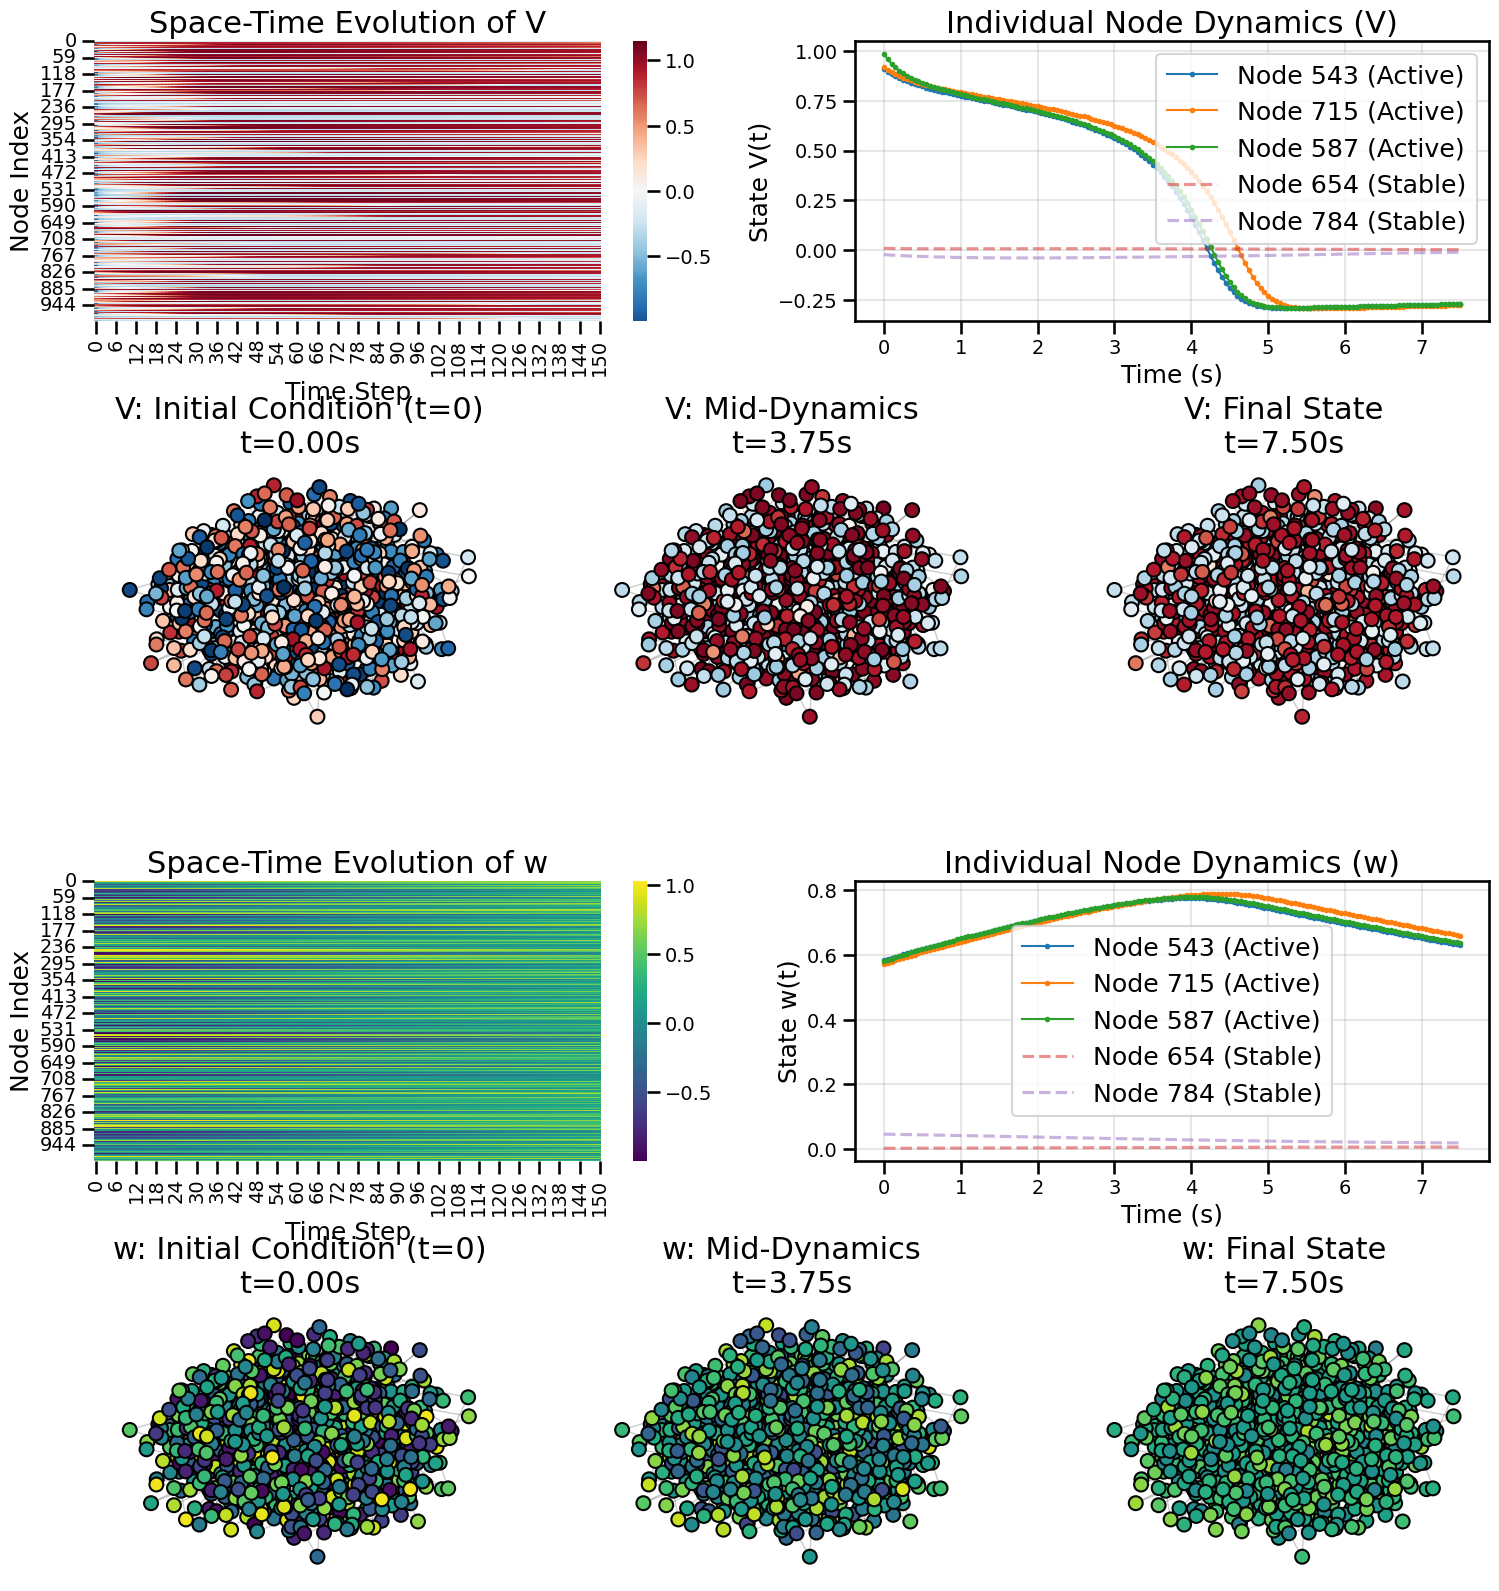
\includegraphics[width=1.0\textwidth]{img/LFNO_FH/dynamics.png}
    \caption{Simulation of the coupled FitzHugh-Nagumo dynamics on a Barabási-Albert graph ($N=1000$, $m=2$). The figure illustrates the space-time evolution, individual node trajectories, and network-wide states for both the activator ($V$, top rows) and inhibitor ($w$, bottom rows) variables, highlighting the distinct non-linear coupled behavior over the $7.5$s simulation window.}
    \label{fig:fhn_dynamics}
\end{figure}

\newpage
\subsection{Training details}
All models were implemented in PyTorch and trained on a dedicated GPU to accelerate tensor operations and spectral transformations. To ensure strict reproducibility, fixed global random seeds ($42$) were explicitly enforced across all data generation and training experiments.

The network parameters were optimized using the Adam algorithm with a weight decay of $10^{-4}$ and a gradient clipping threshold of $1.0$ to ensure numerical stability.
To efficiently manage memory and computational load during the full-horizon rollout, we employed a dual mini-batch strategy: a batch size of $32$ was used for unrolling the trajectory, while a larger batch of $1024$ points was sampled to evaluate the physics-informed residual loss. Both the trajectory tracking and the PDE residual objectives were computed using a relative $L_2$ norm metric to equally balance the contribution of the two FHN variables \footnote{This is consistent with the best found prefactor for the physics loss term $\lambda_{phys}=1$}.

To select the optimal configuration, we performed an automated hyperparameter search using the \textit{Optuna} framework, utilizing a \textit{Median Pruner} to early-stop unpromising trials. Based on this search, the selected hyperparameter configuration for the coupled FitzHugh-Nagumo system was set as follows:
\begin{itemize}
    \item Initial learning rate: $\eta = 7 \cdot 10^{-4}$;
    \item Physics penalty weight: $\lambda_{\text{phys}} = 1.0$;
    \item Initial guesses for the simultaneous system identification of the diffusion coefficients ($D = \varepsilon^2$): we initialized $\varepsilon_{V,\text{init}} = 0.5$ for the activator and $\varepsilon_{w,\text{init}} = 0.3$ for the inhibitor;
    \item Architecture-specific hyperparameters: the spectral layers were configured to retain $330$ Fourier modes with a hidden channel width of $64$.
\end{itemize}

Once the best hyperparameters were identified, the final model was trained for $100$ epochs. The learning rate was scheduled to decay by a factor of $\gamma = 0.5$ every $30$ epochs to refine the convergence. 
To prevent overfitting, we continuously monitored the relative error on the validation set, ensuring that the model weights and the learned physical parameters ($\varepsilon_V, \varepsilon_w$) were saved precisely at the epoch that yielded the lowest validation loss.



\subsection{Results}

The training dynamics of the two-variable LFNO model demonstrate stable and robust convergence. As depicted in the learning curves (Figure \ref{fig:lfno_loss}), both the training and validation losses decrease monotonically on a logarithmic scale. The validation-based checkpointing successfully prevented overfitting, identifying epoch $96$ as the optimal state of the network with the lowest validation error. Since this value is close to the total number of epochs $100$, it is probable that the model could find an even better optimum with a higher number of iterations.

In addition to accurate trajectory prediction, the proposed Operator Learning framework naturally supports \textit{System Identification}. Because the physical diffusion operator is explicitly embedded within the spectral layers, the diffusion coefficients ($\varepsilon_V$ and $\varepsilon_w$) can be simply treated as learnable parameters rather than fixed constants. As illustrated in Figure \ref{fig:lfno_diffusion}, these parameters rapidly converge to their true physical values (accurate to four decimal places) within the very first epochs. The network correctly identifies that the activator $V$ diffuses with $D_V = 0.01$, while accurately recognizing that the inhibitor $w$ is strictly localized ($D_w = 0.00$).

\begin{figure}[htbp]
    \centering
    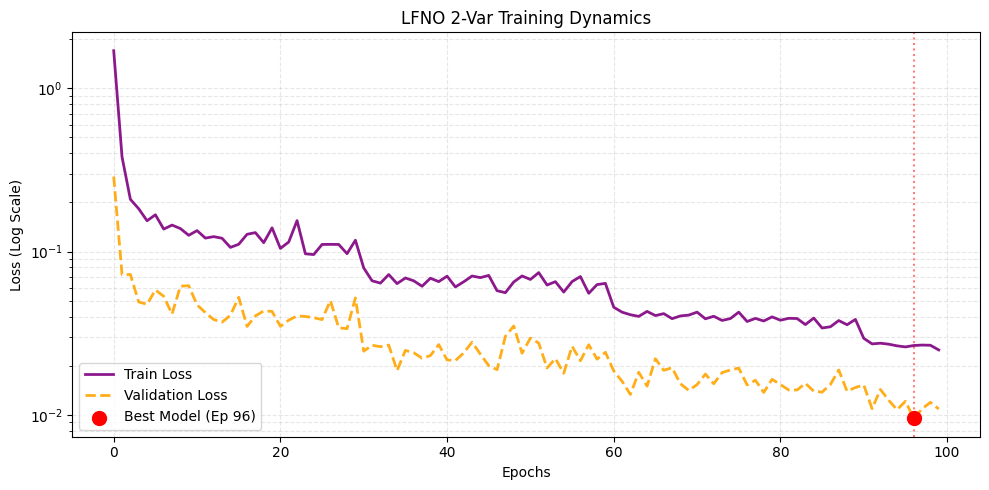
\includegraphics[width=0.85\textwidth]{img/LFNO_FH/loss.png}
    \caption{Training and validation loss curves (MSE). The optimal model weights were extracted at epoch 96 (red marker).}
    \label{fig:lfno_loss}
\end{figure}

\begin{figure}[htbp]
    \centering
    \begin{minipage}{0.48\textwidth}
        \centering
        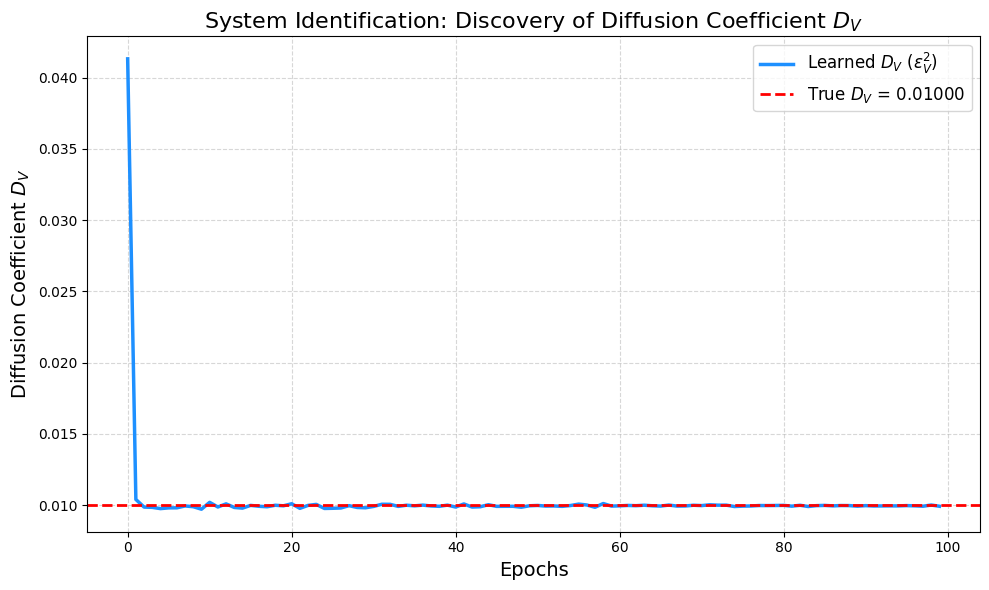
\includegraphics[width=\textwidth]{img/LFNO_FH/Diffusion_coefficient_V.png}
    \end{minipage}\hfill
    \begin{minipage}{0.48\textwidth}
        \centering
        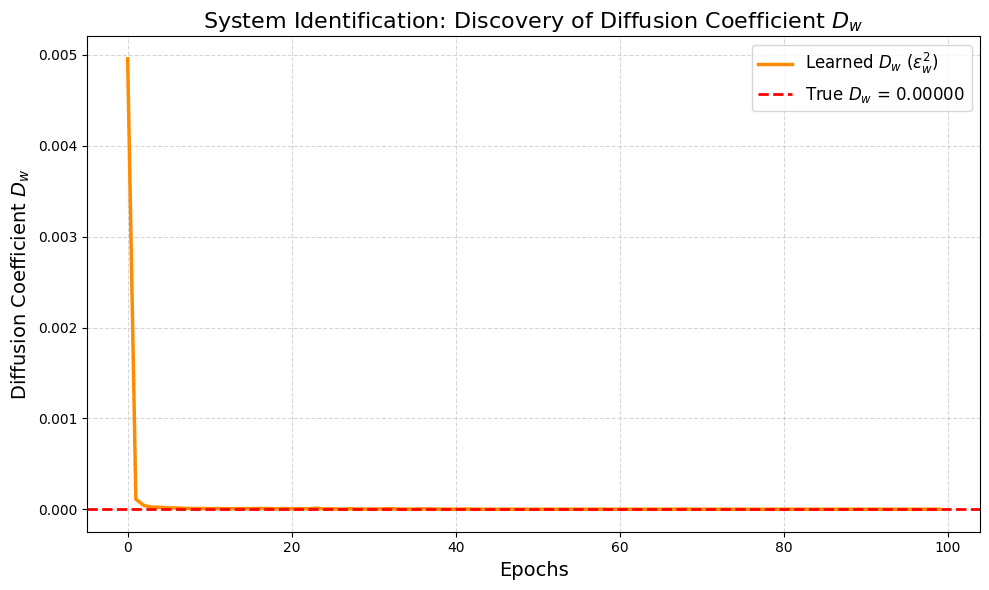
\includegraphics[width=\textwidth]{img/LFNO_FH/Diffusion_coefficient_w.png}
    \end{minipage}
    \caption{System identification of the diffusion coefficients. The network accurately discovers both $D_V = 0.01$ (left) and $D_w = 0.0$ (right) in less than 5 epochs.}
    \label{fig:lfno_diffusion}
\end{figure}

To quantitatively assess the generalization capabilities of the trained model, we evaluated it on a strictly held-out test set. The histogram of the relative $L_2$ errors (figure \ref{fig:lfno_hist}) exhibits a very low mean and variance. The model achieves an outstanding average relative $L_2$ error of just $(0.8 \pm 0.4)\%$, confirming that the LFNO has successfully learned the continuous operator mapping rather than merely memorizing the training trajectories.

\begin{figure}[htbp]
    \centering
    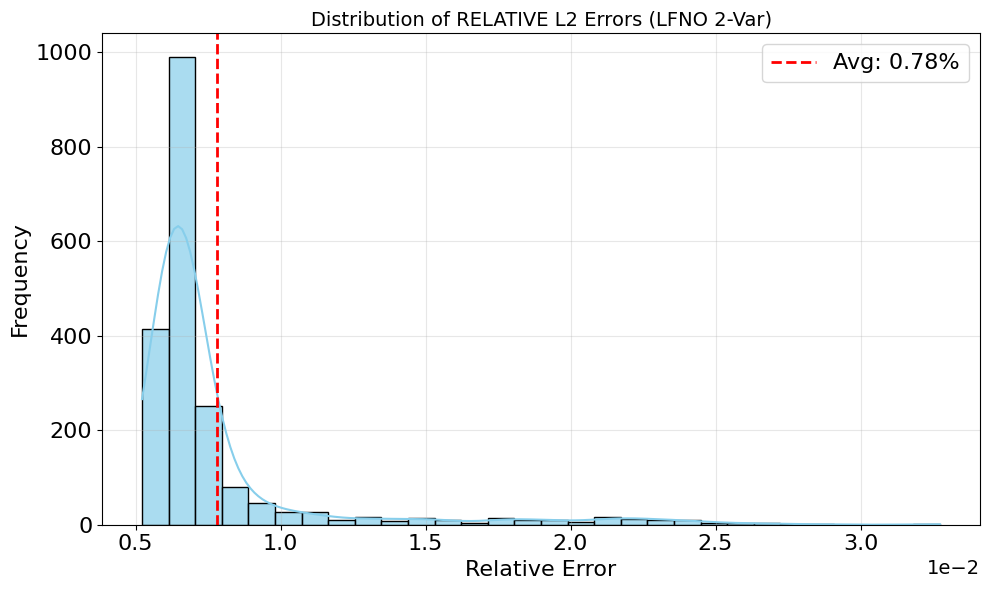
\includegraphics[width=0.75\textwidth]{img/LFNO_FH/Hist_test_set.png}
    \caption{Distribution of the Relative $L_2$ errors evaluated on the unseen test trajectories. The extremely low average error highlights the strong predictive power of the model.}
    \label{fig:lfno_hist}
\end{figure}

Finally, qualitative assessments further validate the numerical results. The space-time heatmaps (Figure \ref{fig:lfno_heatmaps}) show a near-perfect visual overlap between the ground truth and the LFNO predictions for both the activator and the inhibitor variables across the entire network. The absolute error maps remain orders of magnitude lower than the signal amplitude (Mean Absolute Error of $1.09 \times 10^{-3}$ for $V$ and $4.85 \times 10^{-4}$ for $w$). This high fidelity is also evident when zooming in on the continuous dynamics of individual nodes (Figure \ref{fig:lfno_nodes}), where the predicted trajectories (dashed lines) seamlessly track the non-linear physiological behavior of the exact simulated system without any phase shifts or amplitude degradation.

\begin{figure}[htbp]
    \centering
    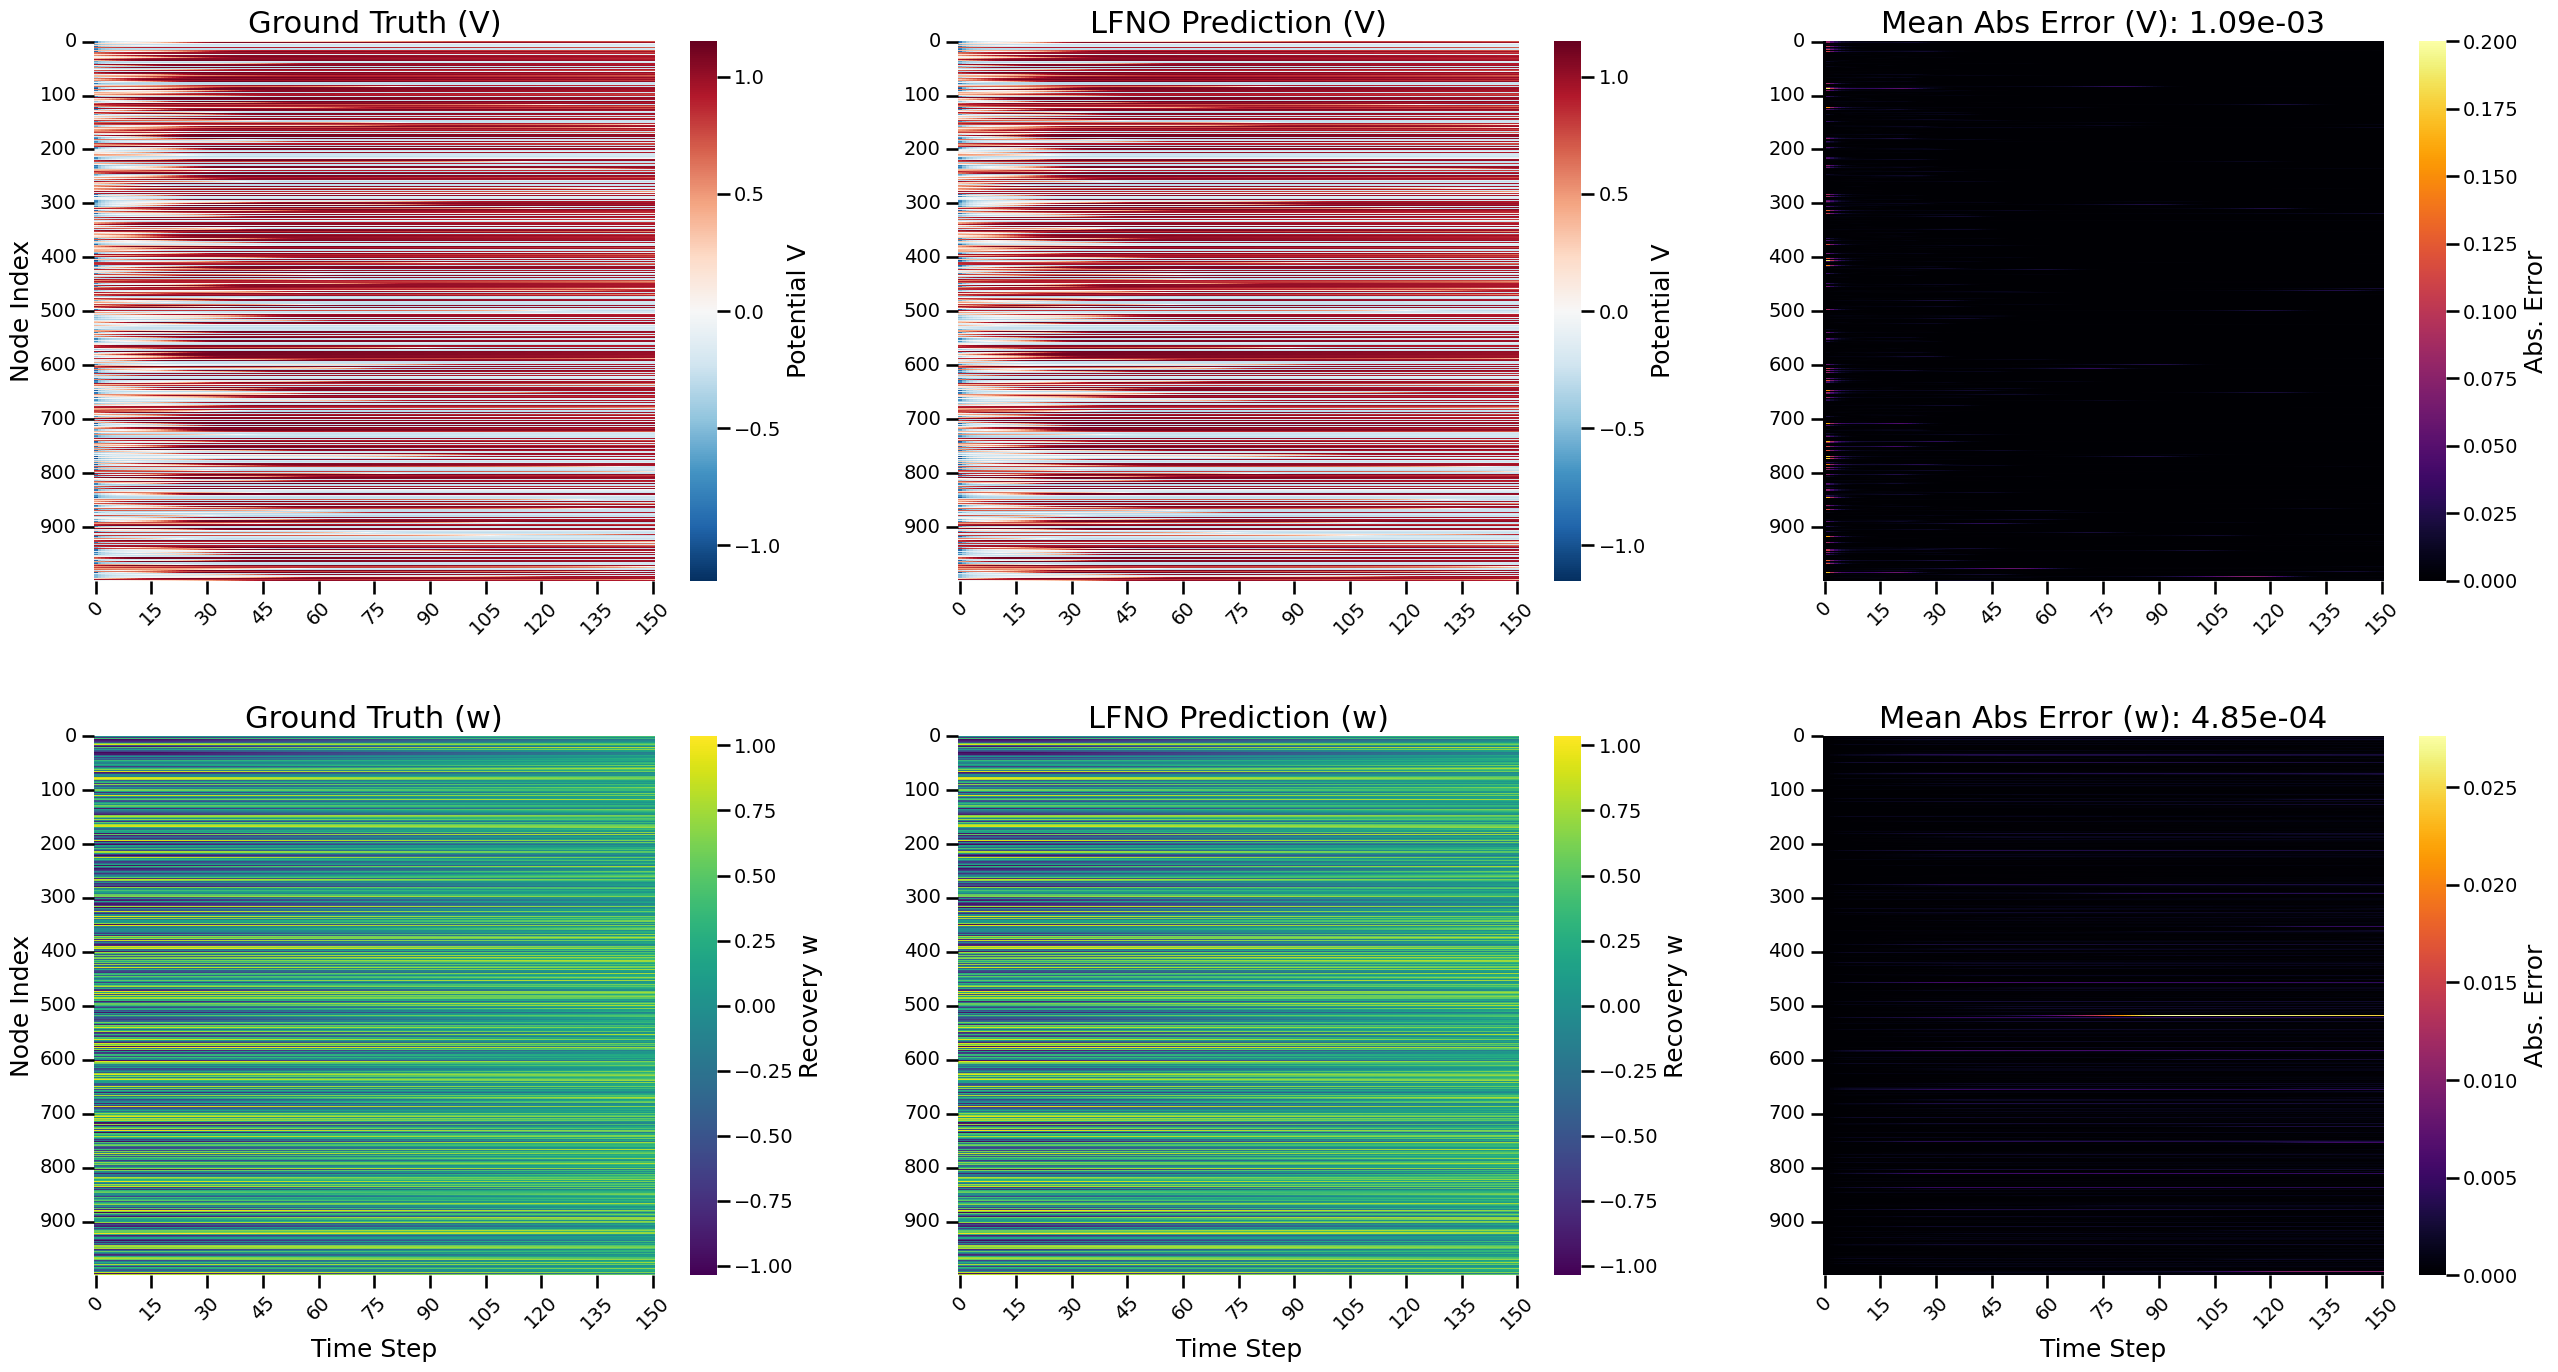
\includegraphics[width=\textwidth]{img/LFNO_FH/Results_test_set.png}
    \caption{Space-time evolution of a typical test trial. The LFNO reconstructions (center) are virtually indistinguishable from the ground truth (left). The absolute error (right) is negligible.}
    \label{fig:lfno_heatmaps}
\end{figure}

\begin{figure}[htbp]
    \centering
    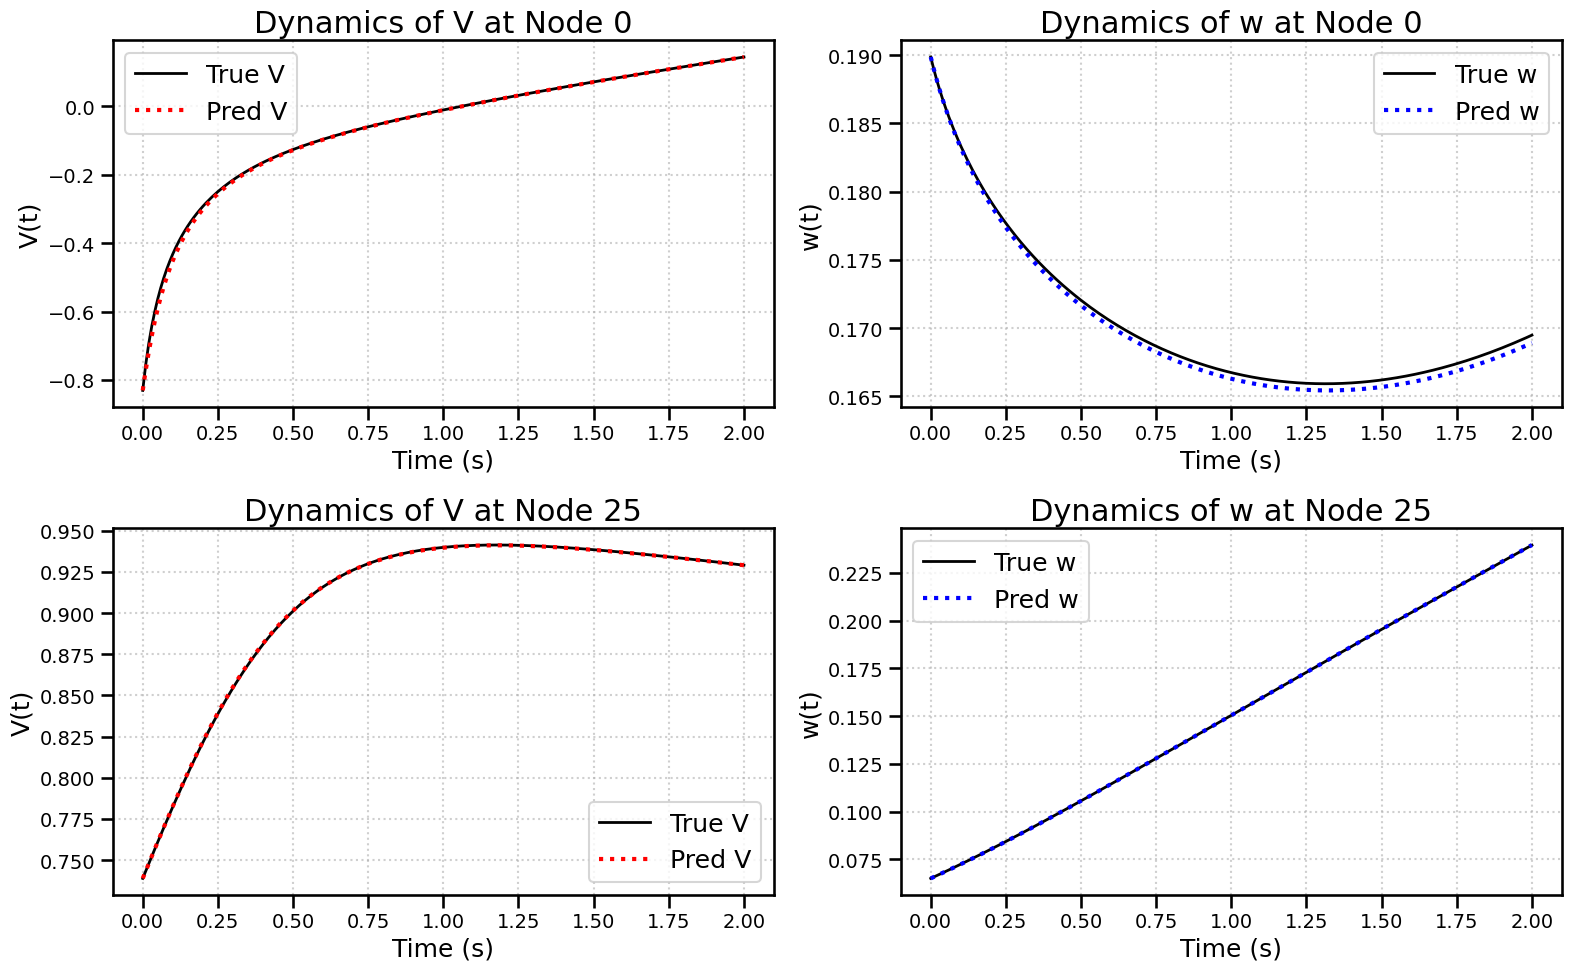
\includegraphics[width=0.9\textwidth]{img/LFNO_FH/Results_single_nodes_test_set_v2.png}
    \caption{Continuous temporal dynamics of individual selected nodes. The LFNO predictions perfectly capture the non-linear, coupled evolution of both $V$ and $w$.}
    \label{fig:lfno_nodes}
\end{figure}

\newpage
\subsection{The inverse problem}
\label{sec:Inverse Problem}

Beyond forward trajectory prediction and system identification of scalar parameters, the proposed architecture allows us to inspect the learned continuous operators. This direction, to our knowledge, has not been explored in the literature yet. 
\newline
Specifically, we can isolate the non-linear reaction terms learned by the network and evaluate them on a discrete 2D grid of $(V, w)$ phase space, comparing them directly against the exact analytical functions $F_V(V, w)$ and $F_w(V, w)$. 

As shown in Figure \ref{fig:lfno_reactions}, the network successfully reconstructs the reaction surfaces. On the naturally explored phase space, the model achieves a relative $L_2$ error of $3.89\%$ for the activator kinetics $F_V(V,w)$ and $1.08\%$ for the inhibitor kinetics $F_w(V,w)$. These low error margins demonstrate that the network is genuinely solving the inverse problem by discovering the underlying governing equations.

However, the metrics reported above are calculated on a grid spanning the specific domain of states predominantly visited during the simulated time horizon, which is not symmetrically distributed. If the learned reaction function $F_V(V,w)$ is evaluated uniformly over the entire $[-1, 1] \times [-1, 1]$ domain, its performance degrades significantly in the negative extreme. In fact if we look at Figure \ref{fig:lfno_reactions2} we can note that the error increases to $23.94\%$ for $F_V(V,w)$, while it remains at $3.45\%$ for $F_w(V,w)$.
\newline
 This limitation is physically grounded: as previously observed in the spatio-temporal dynamics, the $V=-1$ region represents a highly unstable region of the FitzHugh-Nagumo phase portrait. Consequently, the training trajectories rapidly transition away from these states, leaving the neural network with a severe lack of data support in that specific region \footnote{We suppose this doesn't happen around the $V=1$ region both because of the specific initialization and because the gradient is less steep. Morover, increasing the temporal resolution of the simulation may solve this problem. This theory will be subject of future investigations.}. Without sufficient observations, the model cannot accurately extrapolate the cubic curvature of $F_V$, highlighting a fundamental limitation of data-driven inverse modeling in strictly transient or unstable regimes.


\begin{figure}[htbp]
    \centering
    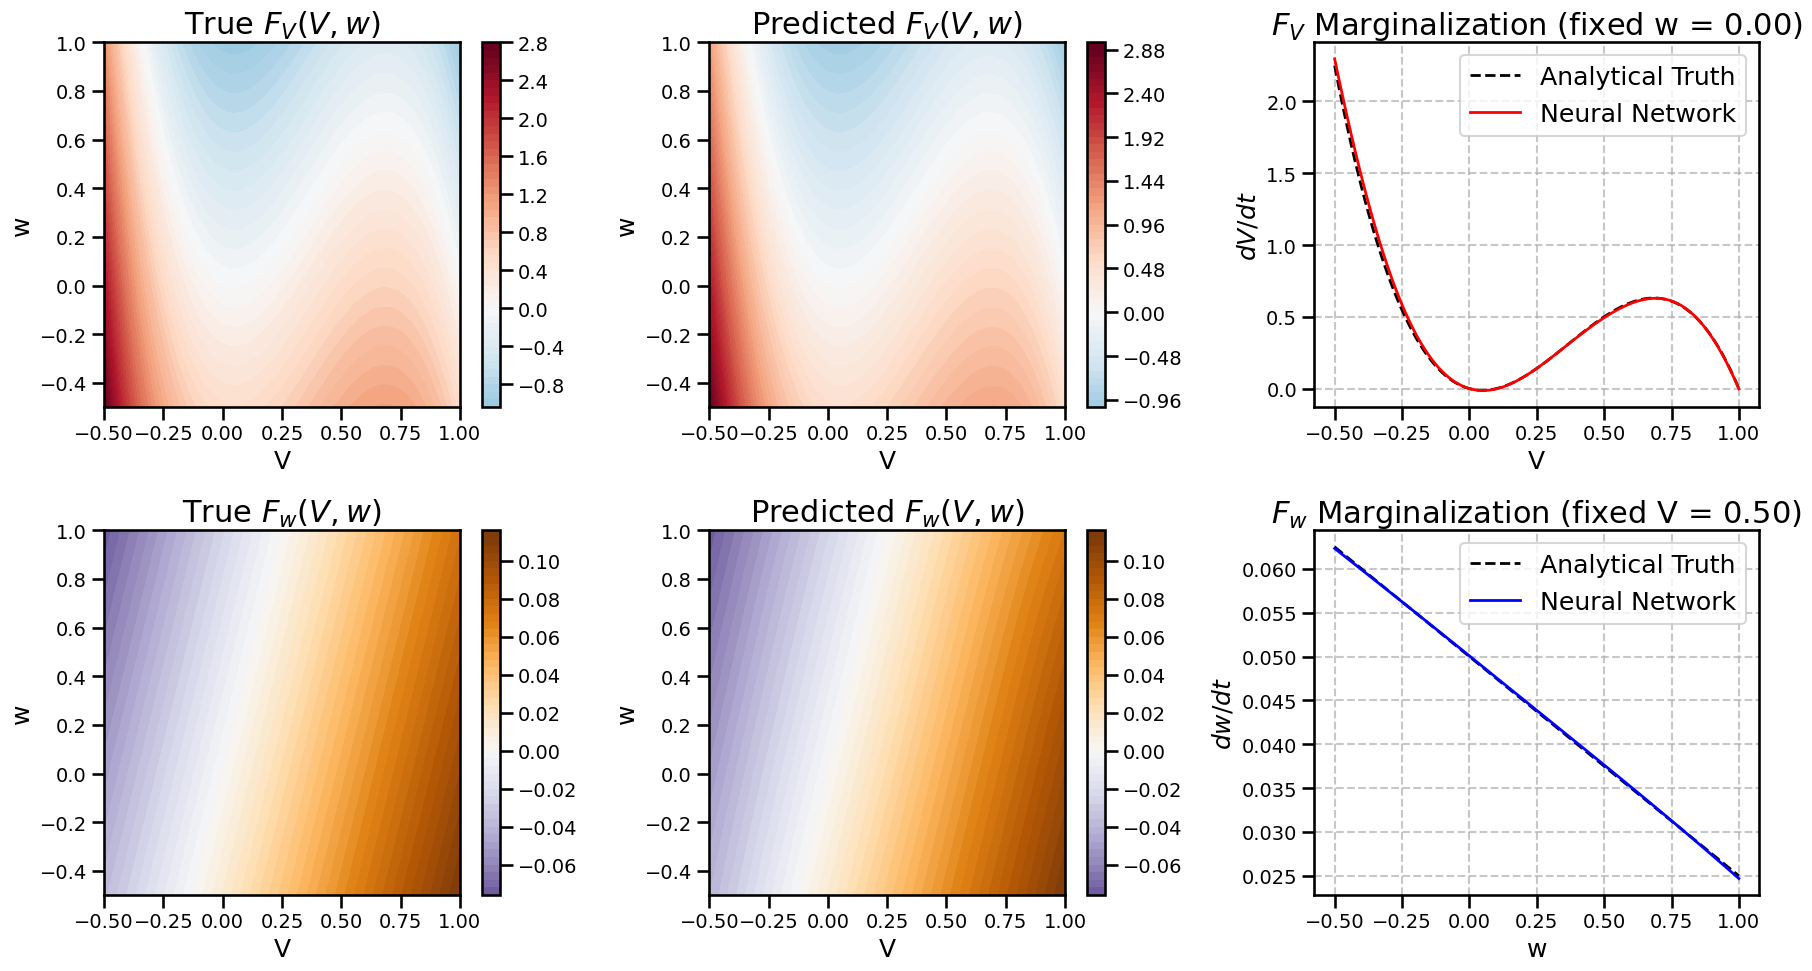
\includegraphics[width=\textwidth]{img/LFNO_FH/Reactions_fit.png}
    \caption{Analytical vs. Learned reaction functions evaluated on the 2D phase space grid $[-0.5,1]^2$}
    \label{fig:lfno_reactions}
\end{figure}

\begin{figure}[htbp]
    \centering
    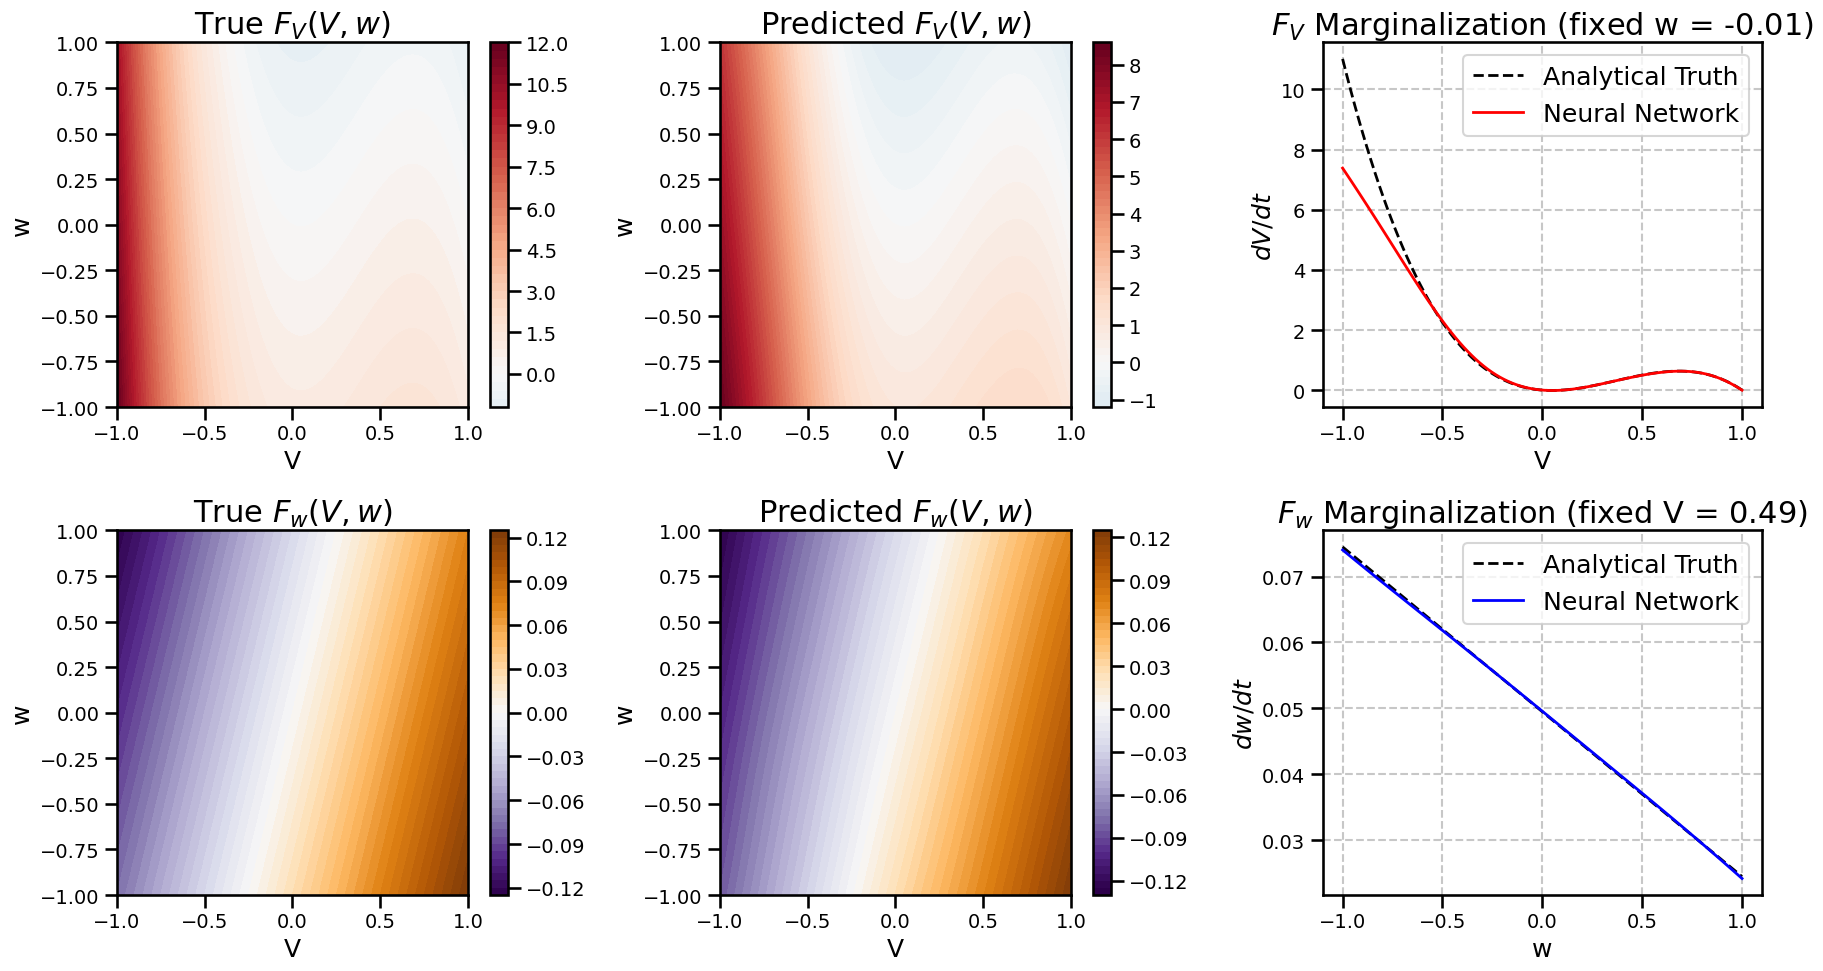
\includegraphics[width=\textwidth]{img/LFNO_FH/Reactions_fit_[-1,1].png}
    \caption{Analytical vs. Learned reaction functions evaluated on the 2D phase space grid $[-1,1]^2$. While the network accurately captures the governing equations in the highly sampled regions, the approximation degrades in the unstable, sparsely sampled domains (e.g., near $V=-1$).}
    \label{fig:lfno_reactions2}
\end{figure}